%%% The main file. It contains definitions of basic parameters and includes all other parts.

%% Settings for single-side (simplex) printing
% Margins: left 40mm, right 25mm, top and bottom 25mm
% (but beware, LaTeX adds 1in implicitly)
\documentclass[12pt,a4paper]{report}
\setlength\textwidth{145mm}
\setlength\textheight{247mm}
\setlength\oddsidemargin{15mm}
\setlength\evensidemargin{15mm}
\setlength\topmargin{0mm}
\setlength\headsep{0mm}
\setlength\headheight{0mm}
% \openright makes the following text appear on a right-hand page
\let\openright=\clearpage

%% Settings for two-sided (duplex) printing
% \documentclass[12pt,a4paper,twoside,openright]{report}
% \setlength\textwidth{145mm}
% \setlength\textheight{247mm}
% \setlength\oddsidemargin{14.2mm}
% \setlength\evensidemargin{0mm}
% \setlength\topmargin{0mm}
% \setlength\headsep{0mm}
% \setlength\headheight{0mm}
% \let\openright=\cleardoublepage


%% Character encoding: usually latin2, cp1250 or utf8:
\usepackage[utf8]{inputenc}

%%%%%%%%%%%%%%%%%%%%%%%%%%%%%%%%%%%%%%%%%%%%%%%%%%%%%%%%%%%%%%%%%%%%%%%%%%%%%%%%
%%% Basic information on the thesis

% Thesis title in English (exactly as in the formal assignment)
\def\ThesisTitle{Comparison of Top trees implementations}

% Author of the thesis
\def\ThesisAuthor{Jiří Setnička}

% Year when the thesis is submitted
\def\YearSubmitted{2018}

% Name of the department or institute, where the work was officially assigned
% (according to the Organizational Structure of MFF UK in English,
% or a full name of a department outside MFF)
\def\Department{Department of Theoretical Computer Science and Mathematical Logic}

% Is it a department (katedra), or an institute (ústav)?
\def\DeptType{Department}

% Thesis supervisor: name, surname and titles
\def\Supervisor{Mgr. Vladan Majerech, Dr.}

% Supervisor's department (again according to Organizational structure of MFF)
\def\SupervisorsDepartment{Department of Theoretical Computer Science and Mathematical Logic}

% Study programme and specialization
\def\StudyProgramme{Computer Science}
\def\StudyBranch{Discrete Models and Algorithms}

% An optional dedication: you can thank whomever you wish (your supervisor,
% consultant, a person who lent the software, etc.)
\def\Dedication{%
I would like to thank my supervisor Vladan Majerech for bringing such interesting
topic, although the topic proved to be more difficult and more challenging than
I~thought. Also I would like to thank my family and friends for patience with me
during writing this thesis.
}

% Abstract (recommended length around 80-200 words; this is not a copy of your thesis assignment!)
\def\Abstract{%
Definition and description of Top trees and introduction of problems solvable by
them including problem of edge 2-connectivity. Definition and description of
Topology trees used as one of the drivers for Top trees.
After the initial descriptions the two top trees implementations are introduced:
one based on self adjusting trees, second based on topology trees.
Comparison of these implementations is done by two experiments. Measurements
are discussed in conclusion -- results corresponds with initial estimates but
with different multiplicative constant than expected.
}

% 3 to 5 keywords (recommended), each enclosed in curly braces
\def\ThesisKeywords{Top Trees, Complexity, Implementation}
%%%%%%%%%%%%%%%%%%%%%%%%%%%%%%%%%%%%%%%%%%%%%%%%%%%%%%%%%%%%%%%%%%%%%%%%%%%%%%%%

% \Subject{\Abstract}
\begin{filecontents*}{\jobname.xmpdata}
\Title{\ThesisTitle}
\Author{\ThesisAuthor}
\Publisher{Charles University}
\Keywords{Top Trees\sep Complexity\sep Implementation}
\end{filecontents*}

%% Generate PDF/A-2u
\usepackage[a-2u]{pdfx}

%% Prefer Latin Modern fonts
\usepackage{lmodern}

% Glyphtounicode cause unicode text easily searchable a copyable from PDF
\input{glyphtounicode}
\pdfgentounicode=1

%% Further useful packages (included in most LaTeX distributions)
\usepackage{amsmath}        % extensions for typesetting of math
\usepackage{amsfonts}       % math fonts
\usepackage{amsthm}         % theorems, definitions, etc.
\usepackage{bbding}         % various symbols (squares, asterisks, scissors, ...)
\usepackage{bm}             % boldface symbols (\bm)
\usepackage{graphicx}       % embedding of pictures
\usepackage{fancyvrb}       % improved verbatim environment
\usepackage[numbers]{natbib}         % citation style AUTHOR (YEAR), or AUTHOR [NUMBER]
\usepackage[nottoc]{tocbibind} % makes sure that bibliography and the lists
			    % of figures/tables are included in the table
			    % of contents
\usepackage{dcolumn}        % improved alignment of table columns
\usepackage{booktabs}       % improved horizontal lines in tables
\usepackage{paralist}       % improved enumerate and itemize
\usepackage[usenames]{xcolor}  % typesetting in color

% Verbatim with syntax highlighting
\usepackage{listings}
\lstset{language=C++,basicstyle=\ttfamily}

\usepackage[footnote,acronym,nomain]{glossaries}
%\setglossarystyle{list}
%\makeglossaries

\usepackage{easy-todo}

\usepackage{asymptote}
\usepackage[format=plain,font=it]{caption}
\usepackage{float}

%% The hyperref package for clickable links in PDF and also for storing
%% metadata to PDF (including the table of contents).
%\usepackage[pdftex,unicode,bookmarksnumbered]{hyperref}   % Must follow all other packages
\hypersetup{unicode}
\hypersetup{breaklinks=true}
%\hypersetup{pdftitle={\ThesisTitle}}
%\hypersetup{pdfauthor={\ThesisAuthor}}
%\hypersetup{pdfkeywords=\Keywords}
\hypersetup{urlcolor=blue}


% Better referencese: \cref with normal first letter and \Cref with uppercase first letter
\usepackage{listings}
\usepackage{cleveref}
% Not so bright color boxes around links:
%\hypersetup{
%    colorlinks,
%    linkcolor={red!50!black},
%    citecolor={blue!50!black},
%    urlcolor={blue!80!black}
%}

% Definitions of macros (see description inside)
%%% This file contains definitions of various useful macros and environments %%%
%%% Please add more macros here instead of cluttering other files with them. %%%

%%% Minor tweaks of style

% These macros employ a little dirty trick to convince LaTeX to typeset
% chapter headings sanely, without lots of empty space above them.
% Feel free to ignore.
\makeatletter
\def\@makechapterhead#1{
  {\parindent \z@ \raggedright \normalfont
   \Huge\bfseries \thechapter. #1
   \par\nobreak
   \vskip 20\p@
}}
\def\@makeschapterhead#1{
  {\parindent \z@ \raggedright \normalfont
   \Huge\bfseries #1
   \par\nobreak
   \vskip 20\p@
}}
\makeatother

% This macro defines a chapter, which is not numbered, but is included
% in the table of contents.
\def\chapwithtoc#1{
\chapter*{#1}
\addcontentsline{toc}{chapter}{#1}
}

% Draw black "slugs" whenever a line overflows, so that we can spot it easily.
\overfullrule=1mm

%%% Macros for definitions, theorems, claims, examples, ... (requires amsthm package)

\theoremstyle{plain}
\newtheorem{thm}{Theorem}
\newtheorem{lemma}[thm]{Lemma}
\newtheorem{claim}[thm]{Claim}

\theoremstyle{plain}
\newtheorem{defn}{Definition}

\theoremstyle{remark}
\newtheorem*{cor}{Corollary}
\newtheorem*{rem}{Remark}
\newtheorem*{example}{Example}

%%% An environment for proofs

%%% FIXME %%% \newenvironment{proof}{
%%% FIXME %%%   \par\medskip\noindent
%%% FIXME %%%   \textit{Proof}.
%%% FIXME %%% }{
%%% FIXME %%% \newline
%%% FIXME %%% \rightline{$\square$}  % or \SquareCastShadowBottomRight from bbding package
%%% FIXME %%% }

%%% An environment for typesetting of program code and input/output
%%% of programs. (Requires the fancyvrb package -- fancy verbatim.)

\DefineVerbatimEnvironment{code}{Verbatim}{fontsize=\small, frame=single}

%%% The field of all real and natural numbers
\newcommand{\R}{\mathbb{R}}
\newcommand{\N}{\mathbb{N}}

%%% Useful operators for statistics and probability
\DeclareMathOperator{\pr}{\textsf{P}}
\DeclareMathOperator{\E}{\textsf{E}\,}
\DeclareMathOperator{\var}{\textrm{var}}
\DeclareMathOperator{\sd}{\textrm{sd}}

%%% Transposition of a vector/matrix
\newcommand{\T}[1]{#1^\top}

%%% Various math goodies
\newcommand{\goto}{\rightarrow}
\newcommand{\gotop}{\stackrel{P}{\longrightarrow}}
\newcommand{\maon}[1]{o(n^{#1})}
\newcommand{\abs}[1]{\left|{#1}\right|}
\newcommand{\dint}{\int_0^\tau\!\!\int_0^\tau}
\newcommand{\isqr}[1]{\frac{1}{\sqrt{#1}}}

%%% Various table goodies
\newcommand{\pulrad}[1]{\raisebox{1.5ex}[0pt]{#1}}
\newcommand{\mc}[1]{\multicolumn{1}{c}{#1}}

%%% Own definitions
\renewcommand{\O}{{\cal O}}
\def\I{\it\aftergroup\/}
\def\Cpp{C{\tt ++}}


% Comment out second line to disable.
\newcommand{\TODO}[1]{}
\renewcommand{\TODO}[1]{{\color{red}\bf TODO: {#1}}}


\parskip=2pt

\input acronyms.tex

%%%%%%%%%%%%%%%%%%%%%%%%%%%%%%%%%%%%%%%%%%%%%%%%%%%%%%%%%%%%%%%%%%%%%%%%%%%%%%%%
% Title page and various mandatory informational pages
\begin{document}
%%% Title page of the thesis and other mandatory pages

%%% Title page of the thesis

\pagestyle{empty}
\hypersetup{pageanchor=false}
\begin{center}

\centerline{\mbox{\includegraphics[width=166mm,type=pdf,ext=.epdf,read=.epdf]{logo-en}}}

\vspace{-8mm}
\vfill

{\bf\Large MASTER THESIS}

\vfill

{\LARGE\ThesisAuthor}

\vspace{15mm}

{\LARGE\bfseries\ThesisTitle}

\vfill

\Department

\vfill

\begin{tabular}{rl}

Supervisor of the master thesis: & \Supervisor \\
\noalign{\vspace{2mm}}
Study programme: & \StudyProgramme \\
\noalign{\vspace{2mm}}
Study branch: & \StudyBranch \\
\end{tabular}

\vfill

% Zde doplňte rok
Prague \YearSubmitted

\end{center}

\newpage

%%% Here should be a bound sheet included -- a signed copy of the "master
%%% thesis assignment". This assignment is NOT a part of the electronic
%%% version of the thesis. DO NOT SCAN.

%%% A page with a solemn declaration to the master thesis

\openright
\hypersetup{pageanchor=true}
\pagestyle{plain}
\pagenumbering{roman}
\vglue 0pt plus 1fill

\noindent
I declare that I carried out this master thesis independently, and only with the cited
sources, literature and other professional sources.

\medskip\noindent
I understand that my work relates to the rights and obligations under the Act No.~121/2000 Sb.,
the Copyright Act, as amended, in particular the fact that the Charles
University has the right to conclude a license agreement on the use of this
work as a school work pursuant to Section 60 subsection 1 of the Copyright Act.

\vspace{10mm}

\hbox{\hbox to 0.6\hsize{%
In \hbox to 2cm{\dotfill} date \hbox to 2cm{\dotfill}
\hss}\hbox to 0.4\hsize{%
signature of the author
\hss}}

\vspace{20mm}
\newpage

%%% Mandatory information page of the thesis

\openright

\vbox to 0.5\vsize{
\setlength\parindent{0mm}
\setlength\parskip{5mm}

{\bf Title:}
\ThesisTitle

{\bf Author:}
\ThesisAuthor

{\bf \DeptType:}
\Department

{\bf Supervisor:}
\Supervisor, \SupervisorsDepartment

{\bf Abstract:}
\Abstract

{\bf Keywords:}
\Keywords

\vss}

\newpage

%%% Dedication

\openright

\noindent
\Dedication

\newpage

\openright
\pagestyle{plain}
\pagenumbering{arabic}
\setcounter{page}{1}


%%% A page with automatically generated table of contents of the master thesis

\tableofcontents

%\listoftodos

%%% Each chapter is kept in a separate file
\chapter*{Introduction}
\addcontentsline{toc}{chapter}{Introduction}

Main aim of this thesis is to provide two different {\I Top Trees}
implementations and to compare them in different situations. Both implementation
were written from scratch in \Cpp{} to provide comparable results.

{\I Top Trees} are not so well known data structure which could be used to
maintain information of some dynamically updated collection of trees. User of
this data structure defines four basic operations, which are used internally
when Top Trees structure is changing. When there occurs some cutting or joining
on underlying trees the structure updates internally stored information using
these user functions.

This data structure could be used for example to dynamically maintain diameter,
center or median (minimizing weighted distance from all other vertices) of given
tree in time $\O(\log N)$ (where $N$ denotes the number of vertices).

Because it is essential to understand how the Top Trees structure works, some
basic principles of the Top Trees structure are introduced in the
\Cref{chap:TopTrees} and some basic principles of Topology trees used in one of
the implementations are introduced in the \Cref{chap:TopologyTrees}. Some
examples of problems, which could Top Trees handle quickly, are listed in
\Cref{chap:Problems} of this thesis.

Basic usage of both implementations and some technical details are the contents
of the \Cref{chap:Implementation}. \Cref{chap:ImplementationSelfAdjusting} and
\Cref{chap:ImplementationTopology} describes details of both implementations.

First implementation of the Top Trees structure is based on article {\I
Self-Adjusting Top Trees} \cite{SelfAdjustingTT} by Tarjan and Werneck. This
implementation promises quick amortized time per operation (with small
constant), but it does not guarantee these times in worst case. This
implementation is described in \Cref{chap:ImplementationSelfAdjusting} of this thesis.

Second implementation is based on article {\I Maintaining Information in Fully-
Dynamic Trees with Top Trees} \cite{TopTrees} by Alstrup, Holm, Lichtenberg and
Thorup and uses Topology trees introduced by Frederickson in
\cite{DSforDynamicallyMaintainingRootedTrees}. This implementation promises time
$\O(\log N)$ in worst-case but with much larger multiplicative constant. This
implementation is described in \Cref{chap:ImplementationTopology} of this thesis.

To compare both implementations it was necessary to perform some experiments on
different problems on different graphs with different sizes. Experiments were
performed on problem of {\I maximum edge weight in tree with interval updates}
(described in section \ref{sec:maximum_edge_weight}) and on problem of {\I edge
2-connectivity} (described in section \ref{sec:edge_2_connectivity}. Details of
these experiments and their setup are described in \Cref{chap:Experiments}.

We expected that the first implementations would have smaller multiplicative
constant than the second one. This expectation turned out to be right and
multiplicative constant for both implementations was measured in
\Cref{chap:Results} together with some results for turning out unnecessary
updates during some operation in the second implementation.

\chapter{Top Trees}
\label{chap:TopTrees}

Top Trees are data structure intended to maintain informations of underlying
dynamically updated forest. They were introduced by Alstrup, Holm, Lichtenberg
and Thorup in {\I Minimizing Diamaters of Dynamic Trees}
\cite{MinimizingDiamatersOfDynamicTrees} in 1997 as variant of the Topology
Trees and they were extended by the same authors in
{\I Maintaining Information in Fully-Dynamic Trees with Top Trees} \cite{TopTrees} in 2003.

\section{Definition}

{\I Top Trees structure} acts as driver for underlying forest. It represents
underlying trees as collection of generalized edges called {\I clusters}. Each
{\I Cluster} represents some subtree in the underlying forest. Only
some of them called {\I root clusters} (which represents whole trees of the
underlying forest) could be directly accessed by the user.

User defines format of the data stored in these clusters and four basic
{\I user functions} \Create, \Destroy, \Join{} and \Split{} used to
manipulate with clusters data. Above that user could define fifth function
\Choose{} which is needed for some use cases but it is not needed for basic
usage.

Then user controls the Top Trees structure by using {\I operations} $\Cut(u,v)$,
$\Link(u,v)$ and $\Expose(u,v)$. Last of them
makes cluster representing the path between vertices $u$ and $v$ a root cluster
(because root clusters are the only clusters of the top tree, whose could be
accessed by the user). The Top Trees structure dynamically updates stored data
in clusters by using user defined functions.

{\I Notation: We will use capitalize form to denote situations where we refer
directly to the defined user functions or to the top trees operations called by
users. When referring to the generic process of joining, splitting or to the
internal procedures related to these processes we will use normal font style.}

%%%%%%%%%%%%%%%%%%%%%%%%%%%%%%%%%%%%%%%%%%%%%%%%%%%%%%%%%%%%%%%%%%%%%%%%%%%%%%%%


\section{Clusters}

As has been said {\I Clusters} are generalized edges. Each cluster has two
{\I boundary vertices} and represents part of the underlying forest between
these vertices. We denote two clusters as {\I connected} if they are edge
disjoint and they share one boundary vertex.

A {\I Clusterization} is division of the underlying forest into clusters such
that each edge is in exactly one cluster. As we mentioned above {\I roots
clusters} are the ones that represents whole trees in the underlying forest
(all edges of their underlying tree are contracted inside and there are no
outgoing edges -- this means that in a clusterization both their boundary
vertices are not connected with any other cluster).

Another special clusters are {\I leaf clusters}. We denote a cluster as a
{\I leaf cluster} in some clusterization if only one of its boundary vertices is
connected to another cluster.

Clusters in the Top Trees structure are organized into binary trees (called
{\I top trees}) where each leaf represents one edge of the underlying forest and
each inner vertex represents contraction of its children. More about this
structure will be discussed later in the {\I Cluster model} subsection. Before
that we need to introduce types of clusters. There are three types of clusters:
\begin{itemize}

\item {\bf Base cluster} -- represents one edge of the underlying forest (and
each edge of the underlying forest has exactly one base cluster, it is 1:1 mapping),
boundary vertices are endpoints of the edge.
This cluster could appear only as leaf in the Top Trees structure.

\item {\bf Rake cluster} -- represents one way how to contract two clusters
with one common boundary vertex. Let's have two clusters $C_1(u,v)$ and
$C_2(v,w)$ next to each other around common boundary vertex $v$ (and let the
$C_1$ be the left one of them in some topological order given for example by
indices of the edges or by some planar embedding).

If the left cluster ($C_1$) is a leaf cluster then we can construct {\I left
rake cluster} by {\I raking} the left cluster ($C_1$) on the right one ($C_2$).
The resulting cluster would have the same boundary vertices as the cluster $C_2$.

If the right cluster ($C_2$) is a leaf cluster then we can, similarly to the
previous case, construct {\I right rake cluster} by {\I raking} the right
cluster ($C_2$) on the left one ($C_1$). The resulting cluster would have the
same boundary vertices as the cluster $C_1$.

\begin{figure}[h]
\centering
\asyinclude{pic/chap01_rake.asy}
\caption{Left and right rake clusters}
\end{figure}

\item{\bf Compress cluster} -- represents other contraction of the two clusters
with one common boundary vertex $v$ into one cluster by attaching first cluster
after the other. Right before compressing the common vertex $v$ must have degree
(number of incident clusters) exactly two. If there are other clusters attached
to the same common boundary vertex they must be firstly {\I raked} onto one of
the compressed clusters.

If boundary vertices of the cluster $C_1$ were $(u,v)$ and boundary vertices
of the cluster $C_2$ were $(v,w)$, the cluster $C=compress(C_1,C_2)$ would have
boundary vertices $(u,w)$ (and we will call it {\I compress cluster
of vertex $v$} and the operation {\I compressing around vertex $v$}).
This cluster also in some way represents the vertex $v$ and we will use it as
{\I handle} of this vertex.

\begin{figure}[H]
\centering
\asyinclude{pic/chap01_compress.asy}
\caption{Compress cluster}
\end{figure}

\end{itemize}

\subsection{Clusters model}

Clusters in the Top Trees structure are organized into binary trees. Leaves of
these trees (Base clusters) represent edges of the underlying trees and each
inner vertex represents contraction of two child clusters into one.

Compress and rake clusters have each of them two children, base clusters are
childless. Each cluster represent subtree of the underlying forest. By
combination of clusters we could represent each underlying tree as one {\I root
cluster}. This whole binary tree of cluster contractions leading to the one root
cluster is called {\I top tree}.

Compress clusters are used to represent paths in the underlying tree -- each
path could be compressed into one {\I compress tree} consisting only of compress
clusters. If there are branches separating from this path, they are firstly
recursively represented as single clusters ({\I rake trees}) and then they are
{\I raked onto} clusters in the path.

Because there are $M$ base clusters for an underlying tree with $M$ edges and
each inner vertex of the corresponding top tree joins two adjacent clusters into
one, there will be $M-1$ inner clusters for representing this underlying tree.

Underlying tree could have (and usually have) many different divisions into
paths and so the underlying tree have many different representations. Crucial
part of the top trees structure is to maintain this representation in some nice
form during updates.

\begin{figure}[H]
\centering
\asyinclude{pic/chap01_top_tree.asy}
\caption{Original tree and corresponding top tree (rake clusters are grey)}
\end{figure}

\subsection{Extended clusters model}

Tarjan and Werneck in \cite{SelfAdjustingTT} suggested that in some cases it may
be useful to modify structure of the clusters and they introduced
{\I foster children} for {\I compress clusters}. In their suggestion a compress
cluster could have up to four descendants -- two normal children and up to two
foster children.

Normal children of a compress cluster are clusters from the compressed path and
foster children are clusters originating from the separating branches. In normal
cluster model they would be raked onto clusters from path and the path would be
compression of these rake clusters.

In this extended model the clusters originating from the separating branches are
firstly combined in so called {\I rake trees} -- there are maximally two rake
trees around each path vertex, one of them is raked from branches on one side of
the path and the second one is raked from branches on the other side of the
path. And these rake trees are connected as left and right foster child of the
compress cluster constructed from this part of the path.

\begin{figure}[H]
\centering
\asyinclude{pic/chap01_rake_trees.asy}
\caption{Rake trees (triangles) around a path, they can be connected as
foster children to compress clusters}
\end{figure}

During computation (\Join{} and \Split{} operations) there is need to use
virtual rake clusters, but it is only $\O(1)$ time complexity per one compress
cluster. We will discuss it later in the first implementation for which this
extended model is used.

\begin{figure}[h]
\centering
\asyinclude{pic/chap01_top_tree_extended.asy}
\caption{Original tree and corresponding top tree with extended clusters model
(foster children are connected by dotted edges)}
\end{figure}

%%%%%%%%%%%%%%%%%%%%%%%%%%%%%%%%%%%%%%%%%%%%%%%%%%%%%%%%%%%%%%%%%%%%%%%%%%%%%%%%


\section{User defined functions}

There are four basic function to manipulate the clusters data which have to
be implemented by users of the Top Trees structure. Then user uses public Top
Trees structure operations and these user functions are used internally when
constructing, destroying or reorganizing clusters.

If user wants to use the \Search{} operation, he has to implement fifth user
function \Choose{} to traverse around the path by choosing children.

Examples of the functions and related problems are given in the \Cref{chap:Problems}.

\subsection{\sc Create}

This function is called when new base cluster is created. It gets reference to
the underlying edge and to the newly created base cluster, populates base
cluster's data based on the underlying edge and runs other user defined
operations according to logic of given problem.

\subsection{\sc Destroy}

Opposite of the \Create{} function. This function is called just before deleting
base cluster. It gets reference to the underlying edge and to the base cluster
which would be destroyed and it could perform some end-of-life operations (like
saving computed data from the cluster).

\subsection{\sc Join}

This function is called during contraction of two clusters into one (compress or
rake) cluster. In the general view it should populate parent cluster with the
data aggregated from contracted child clusters or perform other join-related
operations according to logic of given problem.

It gets a references to both of the contracted clusters and to the newly created
parent cluster with information about their boundary vertices. From boundary
vertices of the parent and both children can be clearly determined if it is
compress or rake cluster (and which one of the children in rake cluster is raked
onto the another one) -- user may or may not use this information according to
the logic of given problem.

\subsection{\sc Split}

Opposite of the \Join{} function. It is called just before removing connection
among parent cluster and its children. This function gets reference to the
parent cluster and both of its children with information about their boundary
vertices. It should distribute data from the parent into children -- notice that
no data could be stored in the parent cluster after the Split operation (because
the parent cluster is deleted after this operation).

The \Join{} and \Split{} operations are frequently called during reorganization of the
Top trees structure -- common pattern is to split everything around changed path
in the top-down manner, reorganize the structure and then join everything in the
bottom-up manner.

\subsection{\sc Choose}

This operation for given cluster with full information (all clusters above it
are splitted -- efficiently this is a root cluster) selects one of its child
clusters. It gets reference to the cluster and its children and returns
reference to one of them. It is used internally by the \Search{} operation.

%%%%%%%%%%%%%%%%%%%%%%%%%%%%%%%%%%%%%%%%%%%%%%%%%%%%%%%%%%%%%%%%%%%%%%%%%%%%%%%%

\penalty-5000 % PRINTHACK

\section{Top Trees operations}

These are the only operations which could user use to manipulate with the Top
Trees structure. In addition to that user could access root clusters and read
informations from them.

\subsubsection{Normalized shape}

Depending on implementation there could be defined a normalized shape of the
Top Trees structure. All operations expect the Top Trees structure in this
normalized shape.

Some operations may corrupt this normalized shape and in that case the correct
shape must be restored prior to the next operation. For both following
implementations an example of such operation is the \Expose{} operation (see
implementation details).

We cannot restore the correct shape right after finishing the operation because
user may need to interact with the Top Trees structure in this corrupted state.
Therefore we have to record that the structure is in corrupted form and we have
to do check and eventually restoration at beginning of each operation. See the
following {\I Restore} operation for more details.

\subsubsection{Handles}

Following operations are defined for pair of vertices of the underlying forest,
but the Top Trees structure operates on (generalized) edges. We need to map
these vertices to clusters.

We want to choose clusters whose in some way represent operations with
vertices. Every cluster represents some path and for given vertex we want to
choose cluster which has this vertex in its path. Also we want that the chosen
cluster could be easily transformed around this vertex. This means that we want
cluster that has chosen vertex as its boundary vertex or common vertex
(if compress clusters).

To accomplish this mapping we define {\I handle} for each vertex of the
underlying forest in this way:

\begin{itemize}
\item Isolated vertex has no handle.
\item If the vertex is a leaf of the underlying tree the
handle for this vertex is the topmost compress (or base) cluster having this
vertex as one of its boundary vertices.
\item Root cluster is handle for its boundary vertices regardless of their
degree in the underlying tree.
\item And finally if the vertex has degree at least two the compress cluster of
this vertex (compress cluster having this vertex as the common boundary vertex)
is the handle of this vertex.
\end{itemize}

One node could be handle for at most three vertices -- two as endpoints and one
as common boundary vertex. To mark handle of a vertex $v$ we will use notation
$N_v$.

With handles we could transform operations with vertices into operations with
clusters.

\subsection{\sc Expose}

Expose is one of the most basic operation. Calling $\Expose(u,v)$ will result in
exposing the $u\dots v$ path (if exists) in the root cluster, which the user
could modify.

Implementation of the expose slightly differs in the first and the second
implementation (first implementation uses splays and splices and the second one
does expose through several splits and joins), but result of both is the
same root cluster (but with possibly different decomposition to subclusters).

See details of both implementations for more information.

\subsection{\sc Restore}

As we mentioned before we may need to keep the Top Trees structure in some
normalized shape. Purpose of this operation is to restore the structure
in such form. Because some operation may corrupt this normalized shape we
call the \Restore{} operation at beginning of all others operations.

To allow the user to modify user functions (\Split, \Join, \dots) for each
operation we will make the \Restore{} callable by the user independently.

In the second implementation we will use this functionality to turn off
expensive updates during the \Expose{} operation, \Restore{} the structure back to the
correct form and before next operation turn the expensive updates back on.

\subsection{\sc Cut}

Operation $\Cut(u,v)$ deletes edge between vertices $u$ and $v$ and reorganizes
the Top Trees structure to reflect this change. Precondition for this operation
is that $u\ne v$ and there exists edge $(u,v)$.

Both implementations user different approaches, but the result is the same --
they remove the $(u,v)$ edge and return root of two new top trees.

\subsection{\sc Link}

The Link operation is an opposite to the \Cut{} operation. Calling $\Link(u,v)$ on
two disconnected vertices joins them by the new edge $(u,v)$. Precondition for
this operation is that $u$ and $v$ are disconnected.

Both implementations user different approaches, but the result is the same --
both top trees are joined by the new edge $(u,v)$ and the cluster of resulting
top tree is returned.

\subsection{\sc Search}

When defined the \Choose{} user function this operation could be used to find
and return specific base cluster.

\todo{Example of search.}

\chapter{Topology Trees}
\label{chap:TopologyTrees}

The Topology Trees data structure introduced by Frederickson
\cite{DSforDynamicallyMaintainingRootedTrees} is used as the basic building
block in the second implementation. We devote this chapter to basic
understanding of how this data structure works and what must be done to use
it in our case.

Basic idea of the Topology Trees is to divide a tree (or in general a forest)
with maximal degree of three into recursive {\I clusters}. Trees with higher
degree has to be firstly {\I ternarized} -- their vertices have to be splitted.
We will discuss the ternarization later, let's suppose we already have
ternarized tree.

A collection of rooted binary trees (called {\I topology trees}) is built from
these recursive clusters, one for each tree in the original forest.

Cluster in topology tree is a set of maximally two nodes (vertices of the
original tree or other topology tree clusters) with edge between them (but
without edges to neighbours) and with maximally three neighbours, better
definition will conclude below. Nodes not connected by edge cannot be in common
cluster, thus clusters represents some contracted subtrees of the original tree.

\section{User interaction}

User of the topology trees could interact with them by using \Cut{} and \Link{}
operations like in the Top trees structure, but there is no \Expose{} operation.
To use it as base for the Top trees structure we will have to implement
\Expose{} differently.

Also note that clusters in topology trees are slightly different than clusters
in top trees. In top trees clusters are generalized edges (with two endpoints)
representing contracted subtree between two vertices, but clusters in topology
trees are generalized vertices (with maximally three outgoing edges).

We will build the Top trees structure based on topology trees in
the \Cref{chap:ImplementationTopology}, now let's introduce details of topology
trees.

{\it Notation: Like in the first chapter we will use capitalize form of the
\Cut{} and \Link{} operations to denote that they are called directly by the
user. Also we will use terms {\sl internal cut} and {\sl internal link} to
denote internal operations that works on a ternarized tree.}

\section{Definition and properties}

\subsection{Topology clusters and clusterization}

A {\I cluster of order $k$} is a set of $k$ nodes connected by edges (there must
be a path from each to each). A {\I clusterization of order $k$} of graph is
division of this graph into clusters that:
\begin{itemize}
\item Each cluster has maximal order $k$.
\item Each vertex of the original graph is contained in exactly one cluster.
\end{itemize}

The {\I Topology clusterization} of a tree (with maximal degree 3) is clusterization
of order 2 whose clusters (called {\I topology clusters}) must meet these conditions:
\begin{enumerate}
\item {\bf Neighbours limit}: Every topology cluster has degree (number of
outgoing edges to neighbours) maximally 3.
\item {\bf Simple crossroads}: Clusters with three neighbours must have order 1 (only one vertex).
\item {\bf Minimality}: There is no cluster that could be merged with its neighbour
without violation these rules.
\end{enumerate}

Because of that there are only 8 types of valid topology clusters:

\begin{figure}[h]
\centering
\asyinclude{pic/chap02_clusters.asy}
\caption{All 8 types of valid topology clusters}
\end{figure}

\subsection{Topology tree}

The {\I topology tree} is a rooted binary tree where each
level of it represents some topology clusterization of the original tree. On the
lowest level each of the original vertices is an independent basic cluster.
These clusters are joined in the first level of topology clusterization,
resulting clusters are contracted and acts as nodes for above level and so on.

Example of topology tree construction and yielding topology tree is on following
figures \ref{fig:topology_tree_construction} and \ref{fig:topology_tree_example}.

Each inner cluster has at most two children on the level below (the clusters
from which is it contracted) and at most one parent (topology clusters without
parent are roots of topology trees). Among these tree edges each topology
cluster is connected with its neighbours on the same level -- each topology
cluster has at most three outgoing edges.

\subsection{Height of a topology tree}

Frederickson in \cite{DSforDynamicallyMaintainingRootedTrees} proved that each
level of topology clusterization has at most $5/6$ clusters of the previous
level. Number of clusters on the lowest level corresponds to the number of
vertices of the original tree (denote it as $N$) and at $k$-th level there are
at most $N\cdot(5/6)^k$ clusters. Therefore the height of the topology tree for
tree with $N$ vertices could be estimated as $\O(\log N)$.

\begin{figure}[h]
\centering
\scalebox{1.3}{\asyinclude{pic/chap02_tree_construction.asy}}
\caption{Example of the topology tree construction. On the bottom level there is
original underlying tree with ternarized vertex $\,e$ (ternarization has no effect
on the construction, for more details see subsection Ternarization).}
\label{fig:topology_tree_construction}
\end{figure}

\begin{figure}[H]
\centering
\asyinclude{pic/chap02_tree_example.asy}
\caption{Resulting topology tree from the previous construction.}
\label{fig:topology_tree_example}
\end{figure}

\section{Updates -- internal cuts and links}

In this section we will assume that we work on a ternarized tree, generic \Cut{}
and \Link{} operations will be discussed below in the ternarization section.

After a change in the underlying forest (adding or removing an edge) we must
update the whole topology trees structure -- after {\I link} (adding edge) two
topology trees are joined into one and after {\I cut} (removing edge) one
topology tree is splitted into two topology trees.

This change has to be propagated on all levels of a topology tree and
corresponding topology clusters (and their neighbours) have to be updated. The
main idea is that this operation should do constant work on each level which
leads to the time $\O(\log N)$ for each operation.

Update process was originally described by Frederickson in
\cite{DSforDynamicallyMaintainingRootedTrees} but my implementation is based on
process described in Martin Mareš's master thesis \cite{DGA} (in Czech). The
process is the same but in the second work was described more clearly.

\subsection{Update process}

Both link and cut starts by modifying the original forest which will break some
constraints in the lowest level of our topology trees. Whole update process
goes from the lowest level up and repairs broken constraints.

Update process work in phases (one phase for level in topology tree) and uses
three lists listed below:
\begin{itemize}
\item {\bf Delete list} -- clusters to be deleted, initially is empty.
\item {\bf Change list} -- clusters whose are changed and needs recomputation, initially
it contains basic clusters at endpoints of the added/removed edge.
\item {\bf Abandon list} -- clusters whose are (for some reason) without parent and
needs some, initially is empty.
\end{itemize}

In each phase update process processes all clusters from all three lists and
prepares lists of clusters from above level for the next phase. When there are
no clusters to process it ends.

Firstly for all clusters from delete list: We delete this cluster (and
disconnect all outer edges) and if it is the only child of its parent we add
parent to the delete list for the next phase, otherwise we add the second child
into current change list, because we need to recompute its neighbours (and
that transitively ensures that parent would get into new change list).

Next for all clusters in change list: If they have sibling (the second child of
their parent) and they are connected with him by edge then everything is correct
-- we only update their neighbours (based on its children neighbours) and add
the parent into next change list (we need to update parent's neighbours too).

If cluster from change list has sibling but they are not connected by edge (for
example the initial state after cut operation) their parent is no longer a
valid cluster -- therefore we add their parent into next delete list and move
both clusters into abandon list (because they are without valid parent).

And finally for all other clusters (rest of change list and abandon list) we do
this process:
\begin{itemize}

\item {\I When cluster had no neighbours we found a new root cluster}
$\rightarrow$ we just save it into list of root clusters.

\item {\I When cluster has three neighbours and one of the neighbours is {\sl single
cluster} (cluster with only one neighbour)} $\rightarrow$ we join them together
under one parent, resulting cluster would have two neighbours. Depending on both
clusters parent there are several options:
	\begin{itemize}
	\item If one of the clusters has parent we reuse it and add this parent
	into next changed list.
	\item If both clusters have parent we choose one, reuse it (adding it
	into next change list) and add second one into next delete list.
	\item If both clusters were without parent we have to create a new one
	and add this new parent into next abandon list.
	\end{itemize}

\item {\I When cluster has three neighbours but no neighbour is single cluster}
$\rightarrow$ we cannot join cluster with any of its neighbours, therefore we
only ensure there is parent of this cluster (if parent exists we add it into
next change list, otherwise we create it and add it into next abandon list).

\item {\I If cluster has degree (number of neighbours) maximally 2 and it has
neighbour without sibling such that degree of cluster plus degree of this
neighbour is maximally 4} $\rightarrow$ We join them together. The resulting parent cluster
will have degree 2 (because we encapsulate the common edge, which we count
twice, into parent cluster). Ensuring the parent cluster is similar as in the
second case. If there is no such neighbour we only ensure that parent of this cluster exists
(similar as in the third case).

\end{itemize}

This process takes $\O(1)$ per level and $\O(\log N)$ for the whole topology tree.

%%%%%%%%%%%%%%%%%%%%%%%%%%%%%%%%%%%%%%%%%%%%%%%%%%%%%%%%%%%%%%%%%%%%%%%%%%%%%%%%

\section{Ternarization of a tree}

One of the things we have to deal with when using Topology trees as an executive
layer for Top trees are degrees of vertices -- the Top Trees structure have to
work on trees of any degree but Topology trees works only on trees with max
degree 3.

We have to {\I ternarize} each vertex -- turning vertex with higher degree into
chain of multiple vertices with degree 3 -- and keep this ternarization during
cuts and joins.

Let's have a vertex of degree $D\ge4$. It could be splitted into chain of
multiple vertices with maximal degree 3 by these simple steps:
\begin{itemize}
\item Create $D - 2$ {\I subvertices} and set their {\I superior vertex} as the
original vertex.
\item Connect subvertices by edges (called {\I subvertice edges}) into one chain (first
and last vertex will have one edge used, inner will have two edges used)
\item Disconnect neighbours from the original vertex and connect them to these
subvertices (there are exactly the right number of free neighbour slots).
\end{itemize}

But the \Cut{} and \Link{} operations in the Top trees works with the original
vertices, we have to build some mapping on internal Topology trees cuts and link
operations.

\subsection{Ternarization during \Cut{} operation}

Both endpoints of the $\Cut(u,v)$ could be processed independently. When cutting on
vertex with degree maximally 3 nothing had to be done and we may simply call
internal cut operation.

When cutting on vertex which is splitted into several subvertices the operation
is more difficult. Firstly we need to find right subvertex which incidents with
the edge. This could be done easily by some list of pointers. After finding the
right subvertex and edge we call the internal cut on this edge, but this
operation decreases degree of this subvertex. According to situation we have to
do several repair steps:

\begin{itemize}
\item {\I If this is inner subvertex of the subvertice chain:} We remove it
from the chain, we need two internal cuts on edges to both neighbours and one
internal link to directly reconnect neighbours.
\item {\I If this is outer vertex of the subvertices chain and there is at least
one inner vertex of the chain (when degree of the original vertex was
at least 5):} We ``steal'' one outer edge from the neighbour (which is
an inner vertex of the subvertice chain) by one internal cut and one internal
link and then we continue as in the first case by removing this inner vertex.
\item {\I If this is outer vertex of the subvertice chain and there is no inner
vertex:} We have to join subvertices into the original vertex. We cut each edge
to neighbour and link it back to the original vertex, finally we cut the edge
between both subvertices and delete these subvertices.

Because degree of the original vertex is 3 after this operation we do exactly
4 internal cuts and 3 internal links.
\end{itemize}

In each case we have to do only constant number of internal cuts and links. All
these inner operations work in the $\O(\log N)$ time so the time complexity of
the whole \Cut{} operation is $\O(\log N)$ (but the multiplicative constant could
be really large).

\subsection{Ternarization during \Link{} operation}

As in the \Cut{} operation both endpoints of the $\Link(u,v)$ could be processed
independently. We firstly need to ensure that both endpoints have degree at
most 2. When linking such vertices we not need to do anything and we just simply
call internal link operation.

When linking vertex with degree 3 or more we need to split it into subvertices
(or add a new subvertex to the existing subvertices chain).

When degree of the vertex was exactly 3 it is not splitted and we have to split
it -- as in the procedure above we create two subvertices, we link them by one
edge and then for all existing neighbours we cut them from the original vertex
and link them to one of the subvertices. One subvertex ends with degree only
2 and this subvertex we use as an endpoint for the main link operation.

Otherwise when vertex is already splitted into subvertices we have to create
a new subvertex and insert it into the subvertices chain. Easiest is to do cut
between the first and the second subvertex in the chain and then two links --
between the first and the new and between the new subvertex and the second subvertex.
Then we use the new subvertex as an endpoint for the main link operation

In each case we have to do only constant number of inner cuts and links. All
these inner operations works in the $\O(\log N)$ time so the time complexity of
the whole \Link{} operation is $\O(\log N)$ (but as in the \Cut's case the
multiplicative constant could be really large).

\chapter{Examples of problems and user functions}
\label{chap:Problems}

In this section there is a list of several problems which could be solved by
Top Trees with small time complexity.

\section{Finding distance between two vertices}

This problem was originally solved in {\I A Data Structure for Dynamic Trees}
\cite{DSforDynamicTrees} by Sleator and Tarjan in 1983 and then it was adapted
for Top Trees by Alstrup, Holm, Lichtenberg and Thorup in \cite{TopTrees}.

{\bf Theorem:} Lets have dynamic collection of weighted trees with link and cut
operations. We could find length of the path between any two vertices (or find
that they are not connected) in $\O(\log N)$ time.

\medskip\noindent
{\bf Proof:} We will maintaing length of the cluster path in every cluster.

\begin{itemize}

\item $\Create$ creates cluster length equivalent to the length of the
underlying edge.

\item $\Join$ of clusters $C_1$ and $C_2$ into $C$ depends on the type of the $C$:
	\begin{itemize}
	\item If $C$ is a compress cluster of $C_1$ and $C_2$:
	Set length of the $C$'s path as sum of the lengths of $C_1$ and $C_2$.
	\item If $C$ is a rake cluster and $C_1$ is raked onto $C_2$:
	Set length of the $C$'s path as length of the $C_2$'s path (and vice
	versa if $C_2$ is raked onto $C_1$).
	\end{itemize}

\item $\Split$ and $\Destroy$ does nothing.

\end{itemize}

After that we could easily get length of the $(u,v)$-path by calling
$\Expose(u,v)$ and reading length from this cluster. Because operations
in user functions are in constant time and \Expose{} takes $\O(\log N)$
operations, we could answer on any such question in $\O(\log N)$ time.

%%%%%%%%%%%%%%%%%%%%%%%%%%%%%%%%%%%%%%%%%%%%%%%%%%%%%%%%%%%%%%%%%%%%%%%%%%%%%%%%

\section{Maximum edge weight between given vertices with interval update}
\label{sec:maximum_edge_weight}

Similarly to the previous problem this problem was originally solved in
\cite{DSforDynamicTrees} and then it was adapted for Top Trees  in
\cite{TopTrees}.

{\bf Theorem:} Let's have dynamic collection of weighted trees with operation of linking,
cutting, updating edge weight and updating edge weight on given path. We could
find maximum edge weight between any two vertices (or find that they are not
connected) in $\O(\log N)$ time.

\medskip\noindent
{\bf Proof:} We can maintain $w_{max}$ in each cluster as maximum weight on this
cluster's path and $w_{extra}$ as weight added to each edge on this path.

\begin{itemize}

\item $\Create$ creates cluster with $w_{max}=w(e)$ where $e$ is the edge for
which is this cluster created. There is no extra weight yet, so $w_{extra}=0$.

\item $\Join$ of clusters $C_1$ and $C_2$ into $C$ depends on the type of the $C$:
	\begin{itemize}
	\item If $C$ is a compress cluster of $C_1$ and $C_2$:
	Set $w_{max}$ as maximum of $w_{max}$ from clusters $C_1$ and $C_2$.
	There is no extra weight, so $w_{extra}=0$.
	\item If $C$ is a rake cluster and $C_1$ is raked onto $C_2$:
	Copy $w_{max}$ from the $C_2$. There is no extra weigh, so $w_{extra}=0$.
	\end{itemize}

\item $\Split$ have to distribute $w_{extra}$ to the children. For $C_i$ children
of splitted $C$ will operations depends on the type of the $C$:
	\begin{itemize}
	\item If $C$ is a compress cluster of $C_1$ and $C_2$:
		\begin{itemize}[$\circ$]
		\item $w_{extra}(C_i)=w_{extra}(C_i)+w_{extra}(C)$
		\item $w_{max}(C_i)=w_{max}(C_i)+w_{extra}(C)$
		\end{itemize}
	\item If $C$ is a rake cluster and $C_1$ is raked onto $C_2$:
	Apply above operation only for $C_2$ (and vice versa only for $C_1$ if $C_2$
	is raked onto $C_1$).
	\end{itemize}


\item $\Destroy$ sets weight of the underlying edge: $w(e)=w_{max}$.

\end{itemize}

Then we could just call $\Expose(u,v)$ and read $w_{max}$ or add to $w_{extra}$
of the root cluster representing the $(u,v)$-path. Everything in time complexity
of an {\sc Expose} operation, which is $\O(\log N)$.

%%%%%%%%%%%%%%%%%%%%%%%%%%%%%%%%%%%%%%%%%%%%%%%%%%%%%%%%%%%%%%%%%%%%%%%%%%%%%%%%

\section{Diameter and center of the trees}

%%%%%%%%%%%%%%%%%%%%%%%%%%%%%%%%%%%%%%%%%%%%%%%%%%%%%%%%%%%%%%%%%%%%%%%%%%%%%%%%

\section{Edge 2-connectivity}
\label{sec:edge_2_connectivity}

In time $\O(\log^4 N)$ by Holm, Lichtenberg and Thorup 2001 in \cite{PolylogarithmicAlgorithmsForConnectivity}

\todo{Do some study.}

%%%%%%%%%%%%%%%%%%%%%%%%%%%%%%%%%%%%%%%%%%%%%%%%%%%%%%%%%%%%%%%%%%%%%%%%%%%%%%%%

\section{Vertex 2-connectivity}

In time $\O(\log^5 N)$ by Holm, Lichtenberg and Thorup 2001 in \cite{PolylogarithmicAlgorithmsForConnectivity}

\todo{Do some study.}

\chapter{Implementation and usage}
\label{chap:Implementation}

As has beeen mentioned in the Introduction both implementation are writtten
in \Cpp. More precisely they are written in \Cpp11 with frequent use of smart
pointers introduced in \Cpp11, which helped a lot with memory handling.

Source code of both implementations is attached to this thesis including
Makefile for easier compiling and testing. Source code is also published on
Github, which may be more pleasant way to explore it or use it in other
projects:

\bigskip
\centerline{\url{https://github.com/setnicka/top-trees}}
\bigskip

\section{Interface of the Top Trees structure}

Both implementations share the same interface which makes them easily
interchangeable.

\todo{interface details}

\section{Testing and Graphviz output}

Both implementations have debugging debugging output showing its current state
in Graphviz format.

Graphviz is open source program which is able to visualize several types of
graphs (tree structures included). Both implementations are able to print
Graphviz script at their standard output and this script could be translated by
Graphviz program to a PDF image.

Currently user is able to visualize state of the structure after each operation
(Cut, Link or Expose) using ... \todo{Graphviz methods}

\chapter{Implementation of Top Trees using self adjusting trees}
\label{chap:ImplementationSelfAdjusting}

This implementation is based on article Self-Adjusting Top Trees
\cite{SelfAdjustingTT} by Tarjan and Werneck and uses the extended clusters
model with foster children discussed in the \Cref{chap:TopTrees}.

\section{Construction}

Tarjan and Werneck in \cite{SelfAdjustingTT} suggested this construction:
\begin{enumerate}
\item Choose root $r$ as a vertex with degree one.
\item Orient all edges in the tree containing vertex $r$ towards the vertex $r$.
\item Divide tree into paths starting in some leaf and continuing along the
direction of the edges -- the first path will end in the root $r$ and became the
{\I root path}, other paths end up being connected to some existing path.
\item Recursively compute clusters to represent each path incident to the
root path and create {\I rake trees} from these incident paths.
\item Create binary tree of compress clusters to represent the root path and
connect rake trees as foster children.
\item If there are some unused vertices of degree one start the process again
from any of these vertices to construct another top tree.
\end{enumerate}

In my implementation I choose equivalent construction but in more recursive
manner. I started the same way by choosing the root $r$ as vertex with degree
one, but I don't divide the tree into paths.

Starting from the second vertex we choose one neighbour as continuation of the
path and recursively called the same function on all other neighbours. Recursion
returns clusters representing each of the subtrees and then they could be
raked into left and right rake trees and saved into this vertex for future use.

When compressing the path into compress clusters we just look into the common
vertex of compressed clusters and if there are saved rake trees we connect them
as left and right foster children.

This construction is easier to implement and gives us ability to better control
the shape of the resulting top tree. By choosing neighbors instead of directing
paths from leafs we could prefer longer paths by choosing deepest neighbors
(we firstly run \gls{dfs} to obtain depths). Longer paths are better contracted
in binary tree structure of compress clusters to obtain lower top tree.

\section{Expose}

Expose in this implementation is based on splaying and splicing whose are used
to bring handles of given vertices to the top of theirs top trees.

Implementation of the Expose operation has two parts: soft and hard expose. Soft
expose is used internally by others operations, hard expose is used only in the
Expose itself.

Before moving forward we will recall some internal structure of top trees with
extended clusters model.

%In the second
%implementation with topology trees the expose is implemented by series of cuts
%and joins and this is described in the \Cref{chap:TopologyTrees} of this thesis. We
%describe here the soft and hard expose from the first implementation as they
%operate directly with the top trees clusters.

\subsubsection{Compress and rake trees}

Because of extended clusters model each top tree consist from independent
{\I compress trees} (only compress clusters as internal nodes) and
{\I rake trees} (only rake clusters as internal nodes).

Whole top tree is one compress tree (which represents the {\I root path}). It
has base clusters as leafs and root of rake trees as foster children (these
foster children are other paths connected to the root path). These rake trees
have rake clusters as theirs internal nodes and base or compress clusters as
theirs leaf. And so on.

This division of the top tree into smaller blocks could be used to expose given
pair of vertices in the root of the top tree. We will use operations of
{\I splay} and {\I splice} introduced by Sleator and Tarjan in
\cite{SelfAdjustingBST}.

\subsubsection{Split and Join operations}

Before doing any operation that changes shape of a top tree all nodes involved
in this operation must be splitted (and all theirs parent on the way to the root
of this tree too). This is crucial because after changing shape of the top tree
a data stored in these nodes may be changed (for example depth of subtree bellow
this node).

Split operations have to be done in top-down manner (starting from the root). The
easiest way how to accomplish this is to have flag in each node if it is
splitted and recursively split parent before splitting current node. All
splitted nodes should be logged into some list to easily join all of them after
completing current operation.

Joining is done in opposite direction, in bottom-up manner (ending in the root).
We will assume that before doing anything with any node during splaying and
splicing operations we firstly split this node and after completing the entire
expose operation we will call join on all splitted nodes.

\subsection{Splaying}

Splaying is originally a heuristic for balancing binary trees which uses an idea
that often used nodes should be near the root of the tree. Each operation (find,
delete, \dots) on a vertex in splay tree is preceded by splaying this vertex
which moves this vertex to the root of the tree.

Splaying is done by rotations or double rotations (which are called {\I zig-zig}
or {\I zig-zag} rotations). That moves target vertex up by one or two levels
leaving all vertices in the right order.

Although some not so often used vertices may be in $\O(n)$ distance from the
root, Sleator and Tarjan in \cite{SelfAdjustingBST} proved that all operations
works in amortized time $\O(\log n)$ per operation.

In the Top Trees structure We will use {\I guarded splays} that works exactly
the same way as normal splays, but it stops splaying when reaching a guard (some
node). Normal splay has as guard root of the whole tree, but we want to do
splays limited only inside compress or rake tree (not to mix compress and
rake clusters).

Implementation of the splay is straightforward. Only noticeable detail (which
Tarjan and Werneck mentioned in the \cite{SelfAdjustingTT}) is that foster
children are not affected by any rotations, they always keep the same parents.

\subsection{Splicing}

Only by splaying we are not able to expose a path containing both given
vertices. And we are not even able to carry compress clusters over rake trees
(because rake trees are connected as foster children under compress trees). For
that we need to change partitioning of the top tree into paths.

Lets take some vertex $v$ which is internal to some path $a,b$ (so there is
compress cluster around this vertex) and which has node representing path $c,v$
in its connected rake tree. We may change partitioning into paths by removing
one half of the original path (for example $a,v$), connect it into rake tree,
removing node representing path $c,v$ from the rake tree and changing the
compress cluster that it now represents path $c,b$.

\todo{Picture of splice}

Splicing is used after splaying and its task is to move cluster, which is leaf
of some rake tree, to the compress tree above it.

Tarjan and Werneck in the \cite{SelfAdjustingTT} only described the main idea in
the general case, but implementations details had to be worked out. I decided
to do {\I left splice} (replacing left child of the compress cluster) which was
original choose of Tarjan and Werneck, but the procedure would work the same
way if we choose to replace the right child.

My implementation does splicing in this way:
\begin{enumerate}
\item Prepare empty lists of left and right neighbors.
\item Starting from given node $N$ go up until reaching node $N_c$ in compress
tree. During that add left and right neighbors into neighbors lists and destroy
old internal nodes of these rake trees.
\item Add left child of the $N_c$ to the appropriate list of neighbors and
connect $N$ as the new left child of the $N_c$ (that makes $N$ part of the above
compress tree).
\item Construct new left and right foster children (rake trees) from left and
right neighbors lists with respecting their order. New internal rake nodes have
to be constructed (and added into list of nodes for joining).
\end{enumerate}

To assure that we do not broke connectivity of $N_c$ with above clusters by
replacing left child we need to check children of the $N_c$. If the above
cluster (parent) is compress cluster, one of boundary vertices is common vertex
of the parent. And if the parent is rake cluster, one of boundary vertices is
the vertex around which is the parent raked. If this connection is in the left
child we need to flip children (otherwise child with the connection would be
moved into rake tree and connection would broke).

This detail was not discussed by Tarjan and Werneck -- they only suggested
transforming top trees into some normalized form which would work for both
splaying and splicing. But they did not mention some corner cases where such
checking and flipping is needed.

\subsection{Soft expose}

Soft expose is the first part of the Expose operation. It is called as
{\I soft\_expose(u,v)} and its target is to bring path $u\dots v$ as subpath into
the root cluster of corresponding top tree (so after soft expose there should
be some path $a\dots u\dots v\dots b$ in the root cluster). Truncating the root
cluster to contain only $u\dots v$ path is quest for the hard expose operation.

Soft expose takes handles of both vertices and brings them to the top of their
top trees. If both vertices are in different components (they are not connected
by a path) both the handles of $u$ and $v$ are brought to the roots of
corresponding top trees using series of local changes in the top trees
(similarly if $u=v$).

When they are in the same component (they are connected by a path) firstly the
handle of $u$ is brought to the root of corresponding top tree. If the current
root cluster is also handle of $v$ we are done, otherwise the handle of $v$ is
brought as close to the root as possible (but not replacing the handle of $u$ as
root).

\subsubsection{Algorithm}

Exact procedure for one vertex (as described by Tarjan and Werneck in
\cite{SelfAdjustingTT}) is following:

\begin{enumerate}
\item Local Splays -- Starting from the handle of given vertex:
  \begin{enumerate}
  \item Splay current node inside compress tree (that makes it root of that compress tree)
  \item If reaching a root cluster (there is no parent) $\rightarrow$ stop the cycle.
  \item Splay parent inside rake tree (parent of a root of a compress tree is always rake cluster).
  \item Take parent of that node (it is compress cluster having this rake tree as foster child)
  and repeat the cycle.
  \end{enumerate}
\item Splices -- Starting from the handle of given vertex splice current vertex and
moving to its parent. That in every step moves handle of the given vertex across
one rake tree to the above compress tree. Finally it moves this handle into the
root compress tree.
\item Global Splay -- Perform splay on the handle of given vertex (now in the
root compress tree) to make it root of this top tree.
\end{enumerate}

Firstly we expose $handle(u)$ using above procedure. After that we expose
$handle(v)$ with $handle(u)$ as the guard (to assure that it remains at the
top). If both vertices (and so both handles) are in different top trees both of
them ends as roots of theirs top trees -- this situation is not interesting
anymore, so we will assume that they are in the same top tree.

Tarjan and Werneck discussed special situation when one of the vertices has
degree one (and its handle is not a compress cluster around this vertex), in
this case they realized that mentioned procedure leads to exposing handle of the
second vertex with first vertex as one of its endpoints.

Another special case, which they did not discussed, is situation when both
vertices have degree one -- in that case before starting procedure for the
second vertex we have to ensure that the base cluster of the first vertex is not
the left child of root cluster (otherwise it would be moved to rake tree when
splicing the handle of the second vertex, what we do not want).

If handles for both vertices are the same there is nothing to do (both handles
are occupied by the root cluster). When they are different the second handle
ends as one of the first handle children. To make hard expose easier we will
assume that this is the right children (otherwise we just flip left and right
children).

And where is path $u\dots v$ located? There are three possibilities (notice that
we are still operating with extended clusters model, where rake trees are
connected as foster children -- in standard top tree model there could be
intermediate rake clusters and the cluster with path $u\dots v$ could be located
deeper):

\todo{Pictures of all three cases}
\begin{itemize}

\item Root cluster itself -- When both vertices has degree one, they are endpoints
of the root cluster and so their handles are represented in the root cluster.

\item Child of the root cluster -- When one vertex has degree at least two its
handle is compress cluster. In that case the root cluster represents some path
$a\dots u\dots v$ or $u\dots v\dots b$ and desired path $u\dots v$ is
represented in its child (assume that it is the right child, otherwise flip them).

Another case when path is in child of the root cluster is when $u$ and $v$ are
connected directly by an edge. In this case the path is represented by base cluster
and so it might be child of some compress cluster.

\item Grandchild of the root cluster -- When both vertices have degree at least
two both handles are represented by compress clusters. Child of the root cluster
is limited from the first side and its again compress cluster (the second handle).
The grandchild of the root cluster is limited from the second cluster and so it
represents our path (let again assume it is the right child, otherwise flip
children).

\end{itemize}

To ensure that the root cluster represents only the path $u\dots v$ we need the
hard expose operation.

\subsection{Hard expose}

Hard expose is the second part of the expose procedure, it follows the soft
expose and its job is to truncate the path in the root cluster that it contains
only the exposed subpath.

Ideal situation is when $u$ and $v$ are endpoints of the root cluster, it is
possible when both of them have degree one or when all others clusters incident
to the root clusters are raked onto the root cluster.

But in general root cluster could represent some path $x\dots y$ with path $u\dots v$
as subpath. In this case we need to temporarily convert ends of this path (paths
$x\dots u$ and $v\dots y$) into rake clusters so the compress tree would represent the
path $u\dots v$ with these ends raked onto this path.

As we discussed at the end of the soft expose operation, wanted subpath may be
located in the root cluster itself, in its (right) child or in its (rightmost)
grandchild.

Tarjan and Werneck (in \cite{SelfAdjustingTT}) came with simple trick -- temporarily
convert compress clusters above wanted cluster (at most two compress clusters as
we realized above) to rake clusters ({\I rakerizing} them). Because we are using
left rake clusters the resulting rake cluster will have the same boundaries as
its right child -- this is the reason why we needed to have cluster with the
wanted path on the right side.

After rakerizing clusters (we have to not forget to split them before the
operation and join them after it) we have the $u\dots v$ path represented in
the root cluster, expose procedure is finished.

But we brought the top tree in some corrupted form by rakerizing (at most two)
compress clusters. Prior the beginning of the next operation (Expose, Link, Cut
or Search) we have to undone this and return the top tree into its original
form, otherwise the amortization arguments would not work.

When rakerizing we save all rakerized compress clusters into some list and
before any other operation (Cut, Link or Expose) we call the Restore operation.
The Restore operation checks this list and if there are some vertices it changes
them back to compress clusters. All that we could do in constant time at start
of every operation.

\section{Cut}

Implementing cut operation is quite easy thanks to the soft expose operation.
First step of the $cut(u,v)$ operation is to do $soft\_expose(u,v)$ which brings
the top tree into state described at the end of the soft expose subsection
-- depending on the degrees of $u$ and $v$ the cluster representing
$(u,v)$ edge will be the rightmost child or grandchild of the root cluster of the
corresponding top tree.

\todo{Picture of cut}

We have to destroy the base node representing $(u,v)$ and remove connection
between these two handles. After that we have to reorganize clusters to ensure
all clusters have both children.

When one of vertices have degree only one we are removing leaf edge and there
will be only one resulting top tree (or even no resulting top tree when both
vertices have degree only one and the whole top tree consists only from this
edge). Otherwise we have to split the top tree in the middle points of the two
compress clusters (whose we bring to the root by soft expose).

Starting from the root we detach the right child of the current cluster -- but
we could not leave the cluster in this form, we need to find new right child.

If there are some nodes in left or right foster children (rake trees) we could
take one leaf from the rake tree (base or compress cluster) and make it the new
right child of the current cluster. When there is only one cluster in the rake
tree it is easy, but what to do if there are clusters?

When taking cluster from the left rake tree we want to get the leftmost one
(or the rightmost one in the right rake tree) to maintain order. We splay on
the chosen clusters parent (which is rake cluster) to make it the root of this
rake tree, or chosen cluster will be the left (right) child of this cluster and
the rest of the rake tree will be the other child. Now we can simply remove this
parent rake cluster, use our chosen cluster as the right child and rest of the
rake tree as the new left (right) foster child.

The last case is when the current compress cluster have not any foster children,
in that case we simply remove this compress cluster and replace it by its left
child.

This whole procedure is done at most twice (third level is the $u,v$ base
cluster itself). It produces (two) new root clusters clusters of the resulting
top trees after cutting the $u,v$ edge.

\section{Link}

Link is similar to the cut operation but in the opposite way. First step during
the $link(u,v)$ operation is bringing both $u$ and $v$ to the top in
corresponding top trees. This could be simply done by calling
$soft\_expose(u,v)$.

Special case is when we are joining solitary vertices. In that case we simply
construct new base cluster and return it as the new top tree.

Otherwise we choose one vertex (and its handle) as the root of the final top tree,
for easier construction we choose the vertex with bigger degree. Then starting
from the second cluster (handle of the second vertex) we firstly move its right
child into one of its foster children (rake trees). If there is no rake tree it
is simple, otherwise we just construct new rake cluster connecting the existing
rake tree as one of its child and the former right child of the current compress
cluster as its another child.

\todo{Picture of link}

After this move we simply connect the new $u,v$ base cluster as right child and we
are done with this (lower) compress cluster. For the root compress cluster we
will do similar procedure with the only difference -- instead of the $u,v$ base
cluster we will connect just modified compress cluster as the right child. This
leads to constructing the final top tree.

\chapter{Implementation of Top Trees using Topology Trees}
\label{chap:ImplementationTopology}

This implementation is based on the article {\I Maintaining Information in
Fully-Dynamic Trees with Top Trees} \cite{TopTrees} by Alstrup, Holm,
Lichtenberg and Thorup. It builds Top trees structure on the base of topology
trees introduced in the \Cref{chap:TopologyTrees}. The update process of
topology trees and some basic overview of top clusters mapping was discussed in
that chapter, there we will introduce some details of joining, splitting and the
\Expose{} operation (\Link{} and \Cut{} operations have been described in the
mentioned chapter).

\section{Mapping top trees clusters}

Usage of Topology trees as backend for Top trees was described by Alstrup, Holm,
Lichtenberg and Thorup in \cite{TopTrees}. They described the need of
ternarization and how to transform operations with the topology clusters to
\Split{} and \Join{} functions used in the Top trees structure.

Outgoing edges acts differently in topology clusters and top trees clusters --
in topology clusters outgoing edges are not parts of topology clusters, but
top trees clusters are based on these edges. Even that this is a major
difference the mapping could be done quite easily.

But before mapping we have to deal with fake subvertices and subvertice edges
added by ternarization.

\begin{figure}[h]
\centering
\asyinclude{pic/chap06_tree_mapping.asy}
\caption[Example of mapping topology tree clusters onto top clusters]
{Example of mapping topology tree clusters onto top clusters -- on base
level there are three base clusters and on other levels there is always one
topology cluster which combines edge cluster with two clusters from lower levels.}
\label{fig:topology_tree_mapping}
\end{figure}

\subsection{Subvertices and subvertice edges from the Top trees perspective}

During ternarization in the \Cref{chap:TopologyTrees} we added additional
subvertices and subvertice edges into into the graph. That is needed by topology
trees but it may be problem for the top trees operations.

Firstly how to deal with subvertices: When performing top trees \Join{} or
\Split{} and joined cluster has subvertex as its endpoint, we use the superior
vertex of this endpoint instead of the original endpoint when passing endpoint
to the \Join/\Split{} user function. From the user's points of view all
subvertices are represented by the original superior vertex.

And how to deal with subvertice edges? Just ignore them -- there are no top
clusters associated with them. When joining topology cluster with subvertice
edge and two children, we just rake these children ignoring the edge.

\subsection{Associated top clusters}

With each topology cluster may be associated at most three top clusters:

\begin{itemize}
\item {\I Edge cluster} -- when there is an normal edge inside the topology cluster.
\item {\I Combined edge cluster} -- joined {\I edge cluster} and cluster from
the first child (when the first child has its own top cluster).
\item {\I Top cluster} for the whole topology cluster (joining {\I combined edge
cluster} and cluster from the second child if there is any).
\end{itemize}

\begin{figure}[H]
\centering
\asyinclude{pic/chap06_associated_clusters.asy}
\caption[Associated top clusters with topology cluster]
{Combination of clusters $a$-$x$ and $y$-$z$ with edge $xy$: Firstly
edge cluster is created, then is combined with the first child cluster and
then is combined with second child cluster.}
\end{figure}


If topology cluster (or recursive its children) contains at least one normal
edge we call it {\I topology top cluster} (because it has associated top
cluster). Otherwise we will call it {\I empty topology cluster}. Originally all
vertices of the original tree are empty topology clusters and by joining them we
create topology top clusters.


\section{Joins and Splits}

$\Join$ and \Split{} (and \Create{} and \Destroy{} for base clusters) are user
defined functions that are called on top clusters with defined endpoints. We
cannot call them directly on topology clusters, so we need to split topology
clusters to associated top clusters and call user defined function on these top
clusters.

The external view of the topology clusters during splitting and joining is
similar as in the first implementation -- when operating on some topology
cluster we have to firstly ensure that this cluster and all of its parents are
splitted. Splitting is done recursively in the top-down manner and all splitted
clusters have to be joined after completing all operations in the bottom-up
manner. This is done by logging all splitted topology clusters into some list
and joining all of them after completing current operation.

\subsection{Joining}

We will recall that if the topology cluster $C$ is not base cluster on the
lowest level it could have one or two children (mark them as $C_1$ and $C_2$).
When joining the $C$ we have to do these operations:
\begin{enumerate}

\item If $C$ has only one child $\rightarrow$ Just copy $C_1$'s {\I top cluster}
(with endpoints) into the $C$'s {\I top cluster} and end.

\item If there is a normal edge between $C_1$ and $C_2$ $\rightarrow$ \Create{}
new {\I edge cluster} from this edge (otherwise initialize dummy one).

\item If the $C_1$ is a topology top cluster:
\begin{itemize}
\item If we created an {\I edge cluster} $\rightarrow$ \Join{} $C_1$'s {\I top
cluster} with the {\I edge cluster} into {\I combined egde cluster} (depending
on $C_1$'s shape set new cluster's endpoints as rake or compress cluster).
\item Otherwise copy $C_1$'s {\I top cluster} into {\I combined edge cluster}
(with updating endpoints).
\end{itemize}
Otherwise just copy {\I edge cluster} into {\I combined edge cluster}.

\item If the $C_2$ is a topology top cluster:
\begin{itemize}
\item If there is valid {\I combined edge cluster} (if $C_1$ is a topology top
cluster or there is a normal edge) $\rightarrow$ \Join{} $C_2$'s {\I top cluster}
with the {\I combined edge cluster} into $C$'s {\I top cluster} (depending
on $C_2$'s shape set new cluster's endpoints as rake or compress cluster).
\item Otherwise copy $C_2$'s {\I top cluster} into $C$'s {\I top cluster}.
\end{itemize}
Otherwise just copy {\I combined edge cluster} into $C$'s {\I top cluster}.

\end{enumerate}

We have done at most two calls to the \Join{} user function and one to the
\Create{} user function.

\subsection{Splitting}

Split procedure is opposite to the join procedure. Endpoints of all top clusters
are correctly set by the join procedure so we have to only do \Split{} and
\Destroy{} operations in the opposite way.

If there is a normal edge in the topology cluster we firstly \Split{} $C$'s
{\I top cluster} into {\I combined edge cluster} and $C_2$'s {\I top cluster}
and then \Split{} {\I combined edge cluster} into {\I edge cluster} and $C_1$'s
{\I top cluster}. Finally just \Destroy{} the {\I edge cluster}.

When there is a subvertice edge just Split $C$'s {\I top cluster} into children
{\I top clusters}. If some of the children is not a topology top cluster we just
do copy instead of \Split{} (like in the join procedure).

We have done at most two calls to the \Split{} user function and one to the
\Create{} user function.


\section{Expose}

The mechanism of the $\Expose(u,v)$ is slightly tricky. Basic idea of the
\Expose{} in the Top trees structure based on topology trees is to leave the
topology trees intact. We only need to split some topology clusters and then
take their inner top clusters and join them into a new structure.

This procedure was basically described by Alstrup et al. in \cite{TopTrees} but
without any details. Here I describe it will all necessary details.

We split all topology clusters in the paths from both exposed vertices to the
root of corresponding topology tree, which gave us $\O(\log N)$ top clusters
splitted around this path (because of the maximal height of a topology tree for
$N$ vertices).

Then we join all these top clusters to construct {\I auxiliary top tree} such
that the root cluster of this auxiliary top tree would be a compress cluster
with two given vertices as its endpoints (and all other clusters raked on its
path).

After finishing \Expose{} we serve the root cluster to the user and he could do
modifications on this root cluster. When it is over we split the auxiliary top
tree, which distributes information from the modified root cluster into splitted
clusters in the original topology tree. Finally we join all splitted clusters
in the topology tree and the operation is finished.

\subsection{Splitting}

Firstly we start will recursive splitting from both given vertices -- better
said from base topology clusters that contains these vertices. We need to split
all clusters that contain them but not as {\I external vertices} and to save
these splitted vertices into {\I chains} whose we will join in the next step.

We have to make clear that {\I boundary vertices} (or endpoints) that we defined
for top trees may be different that {\I external vertices}. More precisely
external vertices are subset of boundary vertices. We defined that each top
cluster has two boundary vertices because we defined top clusters as generalized
edges. But external vertices are only those boundary vertices that are connected
to others clusters.

With definition of external vertices the splitting part is straightforward --
for each cluster (starting from given vertex's base cluster) we check that given
vertex is external vertex (by checking outgoing edges) and if no we split this
cluster.

Notice that all clusters above the first splitted clusters will be splitted too,
because once the vertex stops be external it will never be external again. To
have the full coverage of the tree we have to add the last not splitted cluster
to the chain too (it will be the first cluster in the chain).

Splitted cluster is divided (by at most two call to the \Split{} user function
and one to the \Destroy{} user function) into at most two topology clusters (one
from which we climbed up and second as its sibling) and one edge.

If there is sibling cluster, this sibling has its top cluster and there is a
normal edge, we \Create{} top cluster for this edge, \Join{} this top cluster
with sibling's top cluster (according to previous situation of both siblings we
join them as rake or compress cluster) and then we add them into chain of top
clusters for the next operation. If there is only edge or only sibling's top
cluster (when there is only a subvertice edge) we just add it into chain
directly without joining.

We only need to care not to add sibling that is on the second vertex's path.
For the second vertex the only difference would be that we will stop this
process when we reach already splitted cluster (otherwise we would add some
clusters twice). Splitted clusters for the second vertex will be saved into
separate chain.

\subsubsection{Example of splitted chains}

We will take topology tree from the figure \ref{fig:topology_tree_construction}
(page \pageref{fig:topology_tree_construction}) and let us \Expose(b,f). We will
start splitting clusters from base clusters containing these vertices as you
can see on the figure \ref{fig:chain_clusters_example}.

Firstly we split all clusters above vertices $b$ and $f$. Then starting from the
vertex $b$ we continue up to the moment, when $b$ stops be an external vertex
-- it is in the cluster $c$-$e_2$ where we add the previous cluster ($c$-$b$)
into the chain. Also we should add our sibling $e_1$-$e_2$, but this cluster is
splitted (because it is on the path from $f$ to the root) so we add only the
edge cluster $b$-$e_1$.

Continuing above we add sibling cluster $g$-$h$ combined with edge (so we will
push cluster $e_2$-$h$ into the chain) and that is all for the first vertex.
For the second vertex we continue up until reaching cluster $e_1$-$e_2$, where
$f$ stops be an external vertex. We add previous cluster $e_2$-$f$ and sibling
$e_1$-$d$ to the second chain (notice that we ignore subvertice edge because it
is not a cluster). Above this cluster we hit the path processed by the first run
and thus we end.

\begin{figure}[h]
\centering
\asyinclude{pic/chap06_expose_splitting.asy}
\caption[Splitting clusters into chains]
{Splitting from vertices b and f. Marked clusters will be added into
chains -- notice that they cover all vertices of the underlying tree and with
connecting edges they cover all edges too.}
\label{fig:chain_clusters_example}
\end{figure}

We ended with two chains of clusters: [$c$-$b$; $b$-$e_1$; $e_2$-$h$] and
[$f$-$e_2$; $e_1$-$d$], that have to be joined together. Subvertices
of the same vertex acts from this point of view as the same vertex and therefore
we may act like all occurrences of the $e_1$ or $e_2$ are $e$ (from this point
we will not act with topology tree structure and ternarization is not needed).

\subsection{Chain joining}

During splitting we saved splitted clusters along the paths from both given
vertices and we saved those splitted vertices into two chains. Now we need to
join them. In \cite{TopTrees} Alstrup, Holm, Lichtenberg and Thorup suggested
some joining based on joining point clusters with arbitrary neighbours and then
compressing all remaining clusters on path.

After several tries I decided to do different approach. All clusters in chains
acts like generalized edges so we can build a tree from them and then run
a DFS (deep first search) on this tree.

Our DFS will return computed top cluster for given subtree and will have three
parameters: a current vertex, target vertex and parent cluster (cluster which
was used to move to the current vertex). Target vertex will guide joining of
clusters so that if subtree under current vertex contains target, the returned
cluster will have target as its endpoint.

When joining clusters during $\Expose(u,v)$ we call DFS with parameters
$chainJoin(u,v,NULL)$.

For each vertex $chainJoin(v,target,parent)$ will do:
\begin{itemize}
\item If there is no outgoing clusters (except the $parent$) return only the
$parent$.
\item For all outgoing clusters $C$ (with endpoints $(v,x)$) recursive call
$$childCluster = chainJoin(x,target,C)$$
\item Rake join all child clusters $cluster$ so that if there was a child
cluster with $target$ endpoint all clusters will be raked onto this cluster
(otherwise rake arbitrarily).
\item If $v$ is $target$ rake $cluster$ onto $parent$ and return this cluster.
Otherwise compress $cluster$ with $parent$ and return this cluster.
\end{itemize}


The last cluster is returned to the user. Because paths from both given vertices
to the root cluster has length at most $\O(\log N)$ there were at most $\O(\log
N)$ clusters. Thus the tree used for DFS search has $\O(\log N)$ edges and there
were at most $\O(\log N)$ calls to the \Join{} user function.

Now the structure is in a degraded form and before any other operation it must
be restored.

\subsection{Restore}

Restore is called manually by the user or automatically by all others
operations. If the structure was modified by the \Expose{} there is a topology
tree in the right shape, but with splitted clusters. And also there is an
auxiliary top tree which could contain modified information that should be
distributed into original clusters.

Firstly we need to \Split{} all the clusters in the auxiliary top tree (there
is at most $\O(\log N)$ clusters). Clusters on the last level of the auxiliary
top tree distribute information to the clusters in the original tree.

Now we can delete the auxiliary top tree and then join all the splitted clusters
in the original tree. Because the initial splitting takes $\O(\log N)$ calls to
the \Split{} user function the joining would take the same amount of calls to
the \Join{} user function.

\subsection{Keeping original clusters during \Expose}

Because the original shape of the underlying topology tree remains intact during
the \Expose{} operation we may use it for our benefit. From the user's point of
view we \Split{} some clusters, then we build from them a new top tree and
finally we destroy this new top tree and \Join{} again the same clusters as were
before.

In some use cases there are a lot of informations in the clusters used for
structural changes in the underlying clusters -- for example in the 2-edge
connectivity that we will use as one of our experiments. In that cases it may be
good to turn off some expensive updates during \Join/\Split{} and to turn them
on after the top tree is returned into its original shape.

For that behaviour we need to remember the original values somewhere. User may do this
on it's own (for example by saving this information in edges), but there is an
better approach. Because our interface for all user functions pass them pointers
to the clusters (and the data is stored inside them) we may keep these original
clusters intact after the \Split{} and then pass them to the \Join{} (instead of
newly created empty clusters). We will use this functionality on our experiment
with the 2-edge connectivity.

\chapter{Experiments}
\label{chap:Experiments}

Comparison of both implementations is an important part of the whole thesis
and for objective results multiple tests were needed.

I choose two different problems mentioned in the \cref{chap:Problems}.
First of them is a problem of maximum edge weight between given vertices with
interval updates (described in section \ref{sec:maximum_edge_weight}), which uses
Top trees directly and aims to work in time $\O(\log N)$ per operation. Second
problem is an edge 2-connectivity (described in section \ref{sec:edge_2_connectivity}),
which uses Top trees ``under the hood'' and aims to work in time $\O(\log^4 N)$
per operation. Both problems uses Top trees in different ways.

Another necessary condition of good comparison is to have various input data. In
our case of investigating Top trees behavior with given problems input data
consist of two things:
\begin{itemize}
\item Size and type of the underlying graph (number of edges, degrees of vertices)
\item Strategy of data structure usage (portion of affected edges, proportion of
operation types, \dots)
\end{itemize}

\section{Experiments strategy}

Common scenario for all experiments was introduced. Each experiment was done
for both implementations with the same input data and with increasing input
size. Common scenario:

\begin{itemize}
\item Choose graph size (number of vertices and edges).
\item For each chosen graph size choose multiple random seeds to generate
initial edges and sequence of operations.
\item For each implementation and every generated input run the test and measure elapsed time.
\item Compute average elapsed time and standard deviation for each input size.
\end{itemize}

Python wrapper was used to generate random seeds and to execute testing utilities.
Testing utilities written in \Cpp{} firstly generates all the input data and
sequence of operations, initializes data structures and then began to measure
time and execute the operations.

This procedure was chosen to minimize influence of test functions and to measure
only the time used by Top trees operations.

\vfill\eject %% PRINTHACK

\section{Maximum edge weight experiment}
\label{sec:experiment_maximum_edge_weight}

This problem was described in section \ref{sec:maximum_edge_weight} and it
operates directly on the underlying tree.

For given size $N$ of the tree and number of operations the initial tree with
$N$ edges and $N+1$ vertices was generated. After that the list of operations
was generated (every operation with the same chance) from following operations
list:

\begin{itemize}
\item Add edge -- Choose random two vertices and execute \Link{} operation
(when we choose two vertices in the same top tree the Top trees structure should
return an error).
\item Remove edge -- If there are at least $\frac{7}{10}N$ edges choose random
edge from list of edges and execute \Cut{} operation (we will maintain array of
added edges so every remove operation should be successful), otherwise skip this
operation.
\item Add weight on path -- Execute \Expose{} operation and modify content of
the returned root cluster.
\item Get weight on path -- Execute \Expose{} operation and read content of the
returned root cluster.
\end{itemize}

Every operation executes $\O(1)$ top trees operations and it should take time
$\O(\log N)$, where $N$ is a number of edges. Number of edges during execution
was maintained between $N$ and $\frac{7}{10}N$ to maintain the same asymptotic
complexity.

Both implementations were tested on the same input data. For each implementation
the initial edges and list of operations were generated from the same random
seed. Then the implementation was initialized from the initial edges and time of
this initialization was measured. And finally all the operations were executed
and running time of all operations was measured.

Source code of the library for maximum edge weight is located in the header file
\texttt{include/examples/maximum\_edge\_weight.hpp} and source code of the
experiment itself is in the \texttt{src/experiment\_edge\_weight.cpp} file.

Results from this experiment follows in the section
\ref{sec:results_maximum_edge_weight}.

\vfill\eject %% PRINTHACK

\section{Edge 2-connectivity experiment}
\label{sec:experiment_edge_2_connectivity}

This problem was described in the section \ref{sec:edge_2_connectivity} and it
uses top trees as helper data structure for more complex operations.

Cover informations with incident edges are stored in top clusters and as a
supplement to the top trees structure it holds informations about all nontree
edges and some global counters.

\subsection{Stored data}

Information stored in each top cluster:
\begin{itemize}
\item Cover level of the cluster (maximal level on which is the cluster path
covered), cover edge of this level.

\item Cover informations to be distributed into children on splitting (lazy
propagation of {\it cover} and {\it uncover} operations).

\item Arrays with incident information for both endpoints of this cluster, size
of these arrays is $\O(\log^2 N)$.
\end{itemize}

Outside of the top clusters there are structures associated to the each edge
(because edge may change from tree to nontree and vice versa we need to associate
this structure with each edge) which holds information about level of the edge
and if it is covered by other edges (like the cover information in top
clusters). Each edge have $\O(1)$ information associated with it.

And finally there are global incident counters for each vertex, they takes
$\O(\log^2 N)$ space.

Because there are a lot of other data structures outside of the top trees
structure we cannot use the top trees structure initialization from underlying
base graph, but we must initialize the structure by inserting all the edges one
by one. During experiments the initialization time was measured independently.

\subsection{Generating initial graph and choosing number of edges}

Important decision during generating graph was number of edges. For graph on $N$
vertices we could have up to $\O(N^2)$ edges, but such graph wouldn't be much
interesting for the question of edge 2-connectivity.

We want to have graphs which are not fully 2-connected, but whose have large
2-connected components. During testing graphs with sizes $cN^2$, $N\sqrt{N}$,
$N\log N$ and $cN$ were tested (where $N$ is number of vertices and $c$ some
small constant) and size $3N$ was chosen as an optimal size with the best
ratio of positive and negative queries (graphs with larger number of edges
has more unbalanced ratio of positive and negative queries).

Initial edges of the graph was generated uniformly randomly as pairs of
vertices. During experiment the number of edges of the underlying graph was kept
between $\frac{7}{10}N\log N$ and $\frac{13}{10}N\log N$.

\subsection{Test scenarios}

Possible operations were described in the section \ref{sec:edge_2_connectivity}.
For measuring time two scenarios were introduced. In the first one $70\ \%$ of
operations were queries, $15\ \%$ of them insertions and last $15\ \%$ were deletions.
This experiment aims to simulate some average structure usage with all operations.

Second scenario does only queries to properly measure difference between normal
variant of the second implementation and variant of the second implementation
with disabled expensive updates during queries.

Source code of the library for maximum edge weight is located in the header file
\texttt{include/examples/double\_edge\_connectivity.hpp} and source code of the
experiment itself is in the \texttt{src/experiment\_double\_edge\_connectivity.cpp} file.

Results from this experiment follows in the section \ref{sec:results_edge_2_connectivity}.

\bigskip

The problem of edge 2-connectivity and its solution is much larger problem than
the problem in the first experiment. I tried to implement it in the best way
but my aim was the comparison of the two top trees implementations, not
building universal solution for edge 2-connectivity.

The experiment still has some undefined behavior in some edge cases (for some
random seeds), but it had no effect on comparison -- when some failure occurred
another random seed was chosen.

\chapter{Results}
\label{chap:Results}

Measured data for all experiment together with specification of computers used
for measure them is attached to this thesis. There we will discuss the results.

\section{Maximum edge weight experiment results}
\label{sec:results_maximum_edge_weight}

Experiment described in section \ref{sec:experiment_maximum_edge_weight} was
performed on both implementations and construction time and execution time of
operations were measured. Execution time per one operation is showed in the
following chart.

\begin{figure}[H]
\centering
\hsize=1.1\hsize
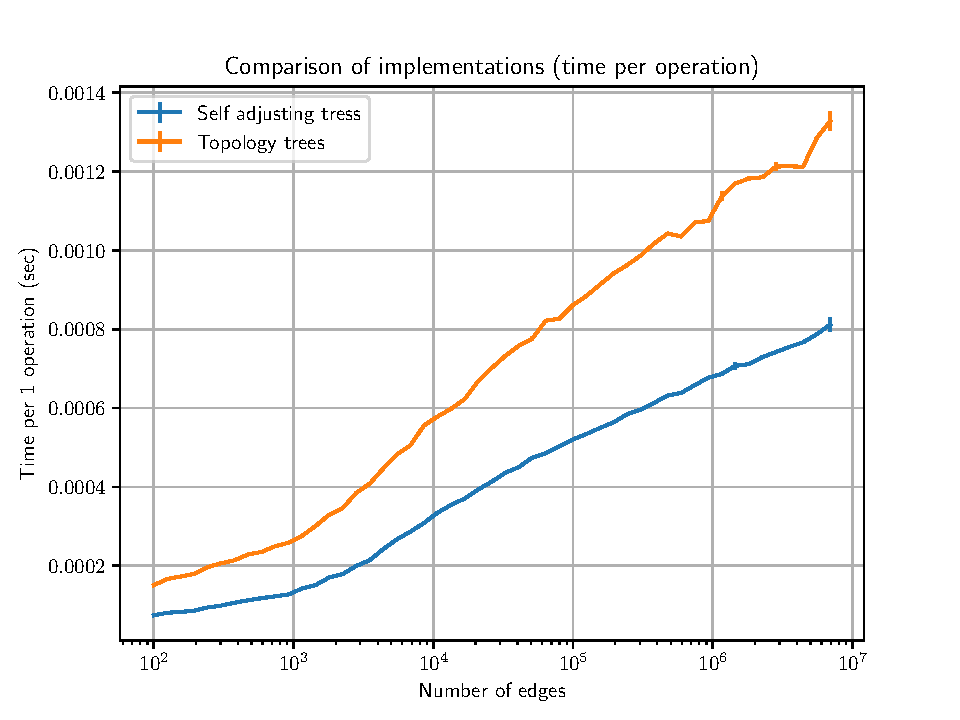
\includegraphics[width=\hsize]{charts/maximum_edge_weight_op.pdf}
\caption{Chart showing time per operation in the maximum edge weight experiment}
\end{figure}

Results show that both implementations have the same asymptotic time complexity
but as have been expected implementation with topology trees have larger
multiplicative constant.

Despite expectations this multiplicative constant is relatively small --
according to measured data the implementation with topology trees for larger
inputs (more than $10^4$ edges) is only $1.58$ to $1.68$ times slower than the
implementation which uses self adjusting trees.

\vfill\eject %% PRINTHACK

\subsubsection{Running time of construction}

Initial construction time measured per one edge of the initial underlying tree
is showed in the following figure. It shows some anomaly for small number of
edges (see bigger standard deviation in the beginning) but from tree size of
$10^4$ edges it stabilizes.

It shows that the implementation based on self adjusting trees could initialize
in approximately half time than the implementation based on topology trees,
which corresponds to time per operation in the previous chart.

\begin{figure}[H]
\centering
\hsize=1.1\hsize
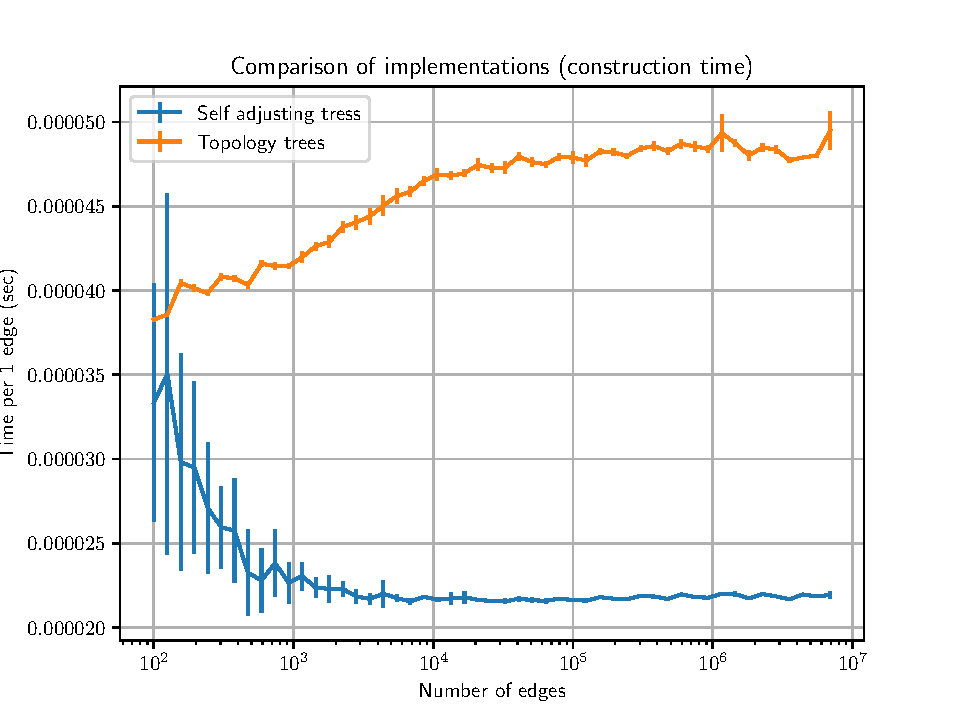
\includegraphics[width=\hsize]{charts/maximum_edge_weight_construction.pdf}
\caption{Chart showing construction time per one edge in the maximum edge weight
experiment}
\end{figure}

\vfill\eject %% PRINTHACK

\section{Edge 2-connectivity experiment results}
\label{sec:results_edge_2_connectivity}

Similarly to the previous experiment the experiment described in the section
\ref{sec:experiment_edge_2_connectivity} was performed on both implementations
(on second with normal updates and with expensive updates turned off during
query). Construction time (time to insert all initial edges) and execution time
of all operations and execution time on only query operations were measured.

\subsubsection{Running time of all operations}

Firstly analyze the running time of normal operations. As you can see on the
following chart, all implementations have the same asymptotic complexity (they
should operate in $\O(\log^4 N)$). The implementation which uses self adjusting
trees has the lowest multiplicative constant as have been expected.

\begin{figure}[H]
\centering
\hsize=1.1\hsize
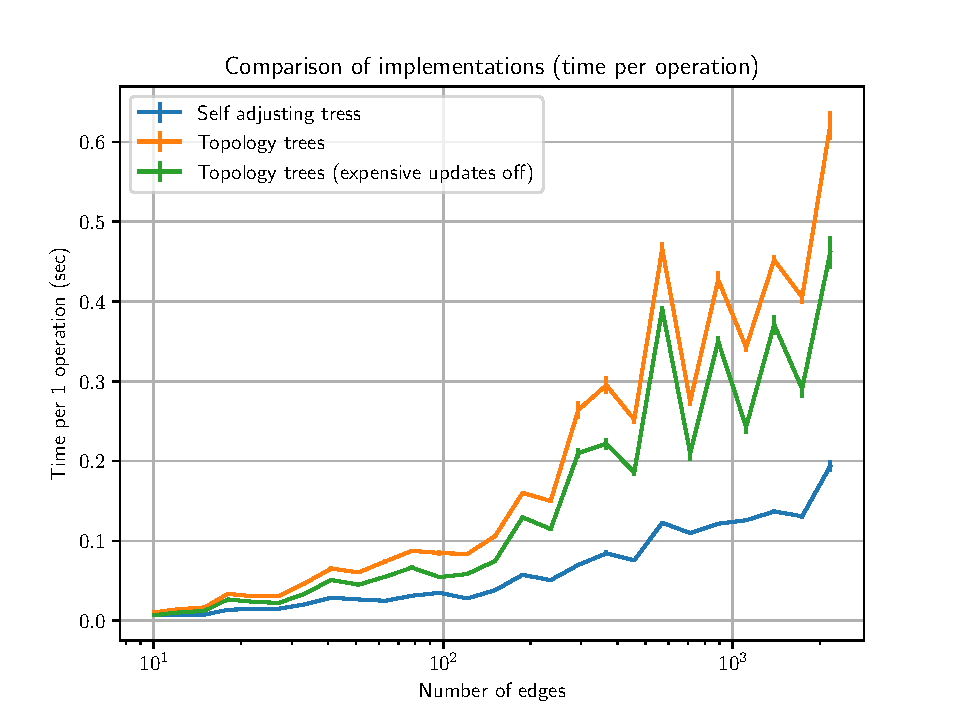
\includegraphics[width=\hsize]{charts/double_edge_connectivity_op.pdf}
\caption{Chart showing time per any operation in the edge 2-connectivity experiment}
\end{figure}

The implementation with topology trees is $2.2$ to $3.5$ times slower than the
implementation which uses self adjusting trees. This multiplicative constant is
larger than the same multiplicative constant in the first experiment.

Mark multiplicative constant from the experiment
\ref{sec:results_maximum_edge_weight} as $C$. Expected value for the
multiplicative constant in this experiment would be $C^3$ (because operations in
this experiment have asymptotic time complexity of $\O(\log^3 N)$ or $\O(\log^4
N)$), but measured multiplicative constant for this experiment is lower. The
difference against the expectation is probably caused by processor caches --
updates in the edge 2-connectivity experiment operates on arrays in the clusters
in sequential order and this cause less cache misses.

Another interesting observation is that turning of expensive updates during
queries have lowers the running time only about 30 \% although the ratio of
queries was 70 \% in all the experiments -- so the most time is spent in the
insertions and deletions of edges.

\subsubsection{Running time of only queries}

In some uses there might be crucial to quickly answer on queries and other
updates may be slower. The second experiment executed only queries and measured
their running time.

\begin{figure}[H]
\centering
\hsize=1.1\hsize
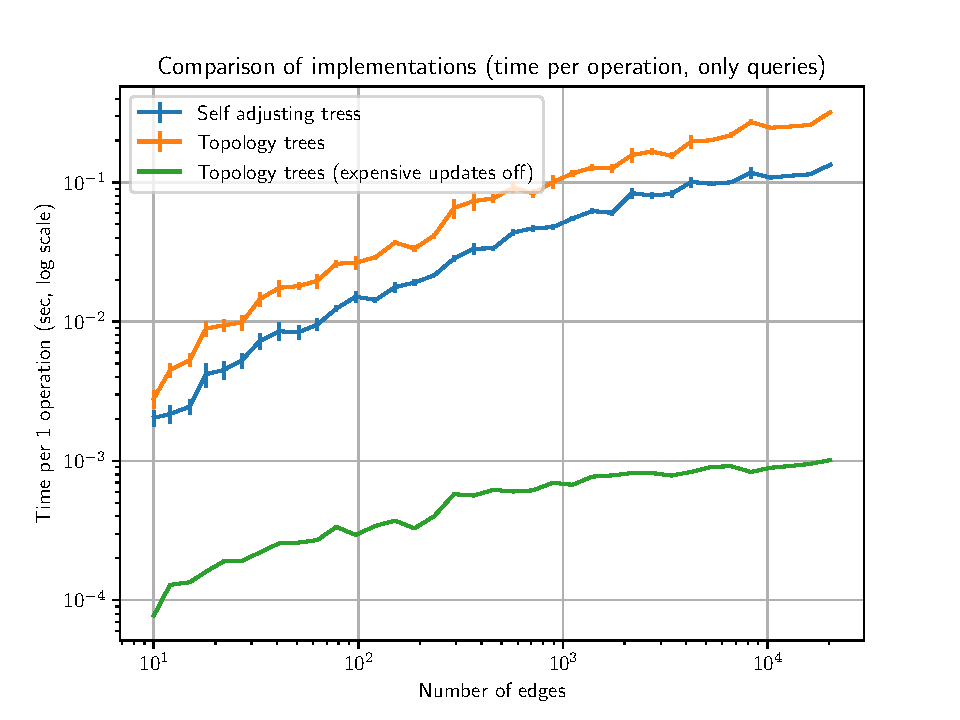
\includegraphics[width=\hsize]{charts/double_edge_connectivity_op_queries.pdf}
\caption{Chart showing time per query in the edge 2-connectivity experiment}
\end{figure}

As you can see on the above chart (it has logarithmic scale on the time axis)
the implementation where we could turn off expensive updates during query --
topology trees implementations -- is the absolute winner. Time complexity of
the implementation without expensive updates is asymptotically lower than the
time complexity of any other implementation.

\subsubsection{Running time of construction}

Construction in this problem cannot be done in one step from some underlying
tree, but it has to be done by sequentially inserting all the edges from the
underlying graph. Thus time of construction of graph with $M$ edges is time of
sequential insertion of $M$ edges into the empty structure.

\begin{figure}[H]
\centering
\hsize=1.1\hsize
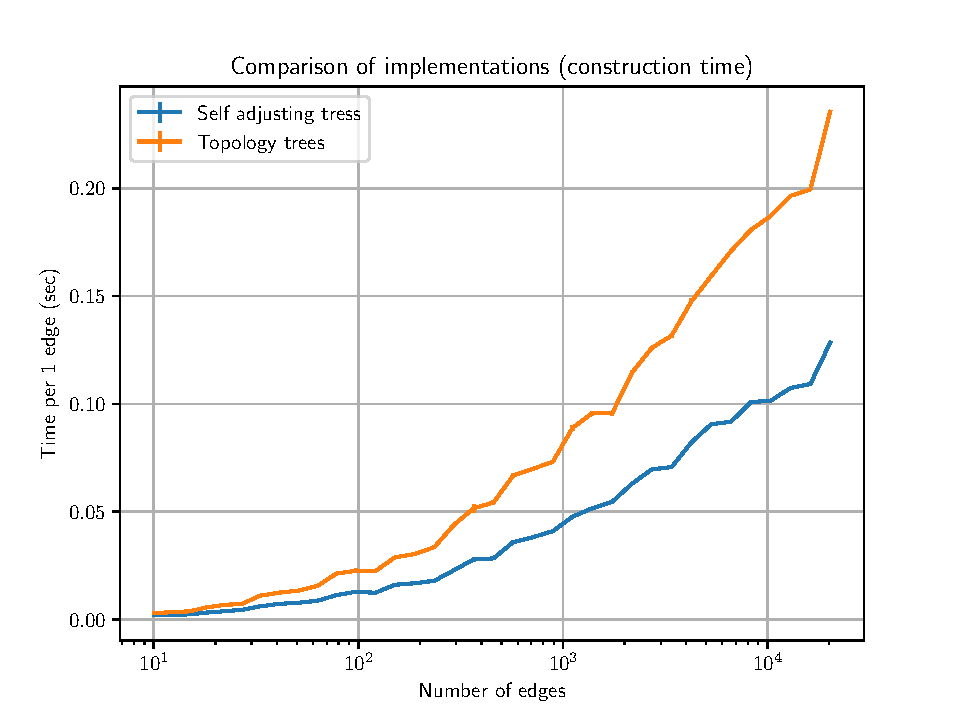
\includegraphics[width=\hsize]{charts/double_edge_connectivity_construction.pdf}
\caption[Chart of construction time per edge in the edge 2-connectivity experiment]
{Chart showing construction time per one edge in the edge 2-connectivity experiment}
\end{figure}

As you can see the construction time is similar and as have been expected the
implementation which uses topology trees is slower. According to measurement
it is $1.7$ to $1.9$ times slower than the construction of the implementation
which uses self adjusting trees.

Not so good result is that the construction time per one edge grows with the
graph size and from some size it starts to be unsuitable for real use. For
production use it would need some construction method like the maximum edge
weight problem.


\chapter*{Conclusion}
\addcontentsline{toc}{chapter}{Conclusion}


%%% Bibliography
%%% Bibliography (literature used as a source)
%%%
%%% We employ bibTeX to construct the bibliography. It processes
%%% citations in the text (e.g., the \cite{...} macro) and looks up
%%% relevant entries in the bibliography.bib file.
%%%
%%% The \bibliographystyle command selects, which style will be used
%%% for references from the text. The argument in curly brackets is
%%% the name of the corresponding style file (*.bst). Both styles
%%% mentioned in this template are included in LaTeX distributions.

% \bibliographystyle{plainnat}    %% Author (year)
\bibliographystyle{unsrt}     %% [number]

\renewcommand{\bibname}{Bibliography}

%%% Generate the bibliography. Beware that if you cited no works,
%%% the empty list will be omitted completely.

\bibliography{bibliography}

%%% If case you prefer to write the bibliography manually (without bibTeX),
%%% you can use the following. Please follow the ISO 690 standard and
%%% citation conventions of your field of research.

% \begin{thebibliography}{99}
%
% \bibitem{lamport94}
%   {\sc Lamport,} Leslie.
%   \emph{\LaTeX: A Document Preparation System}.
%   2nd edition.
%   Massachusetts: Addison Wesley, 1994.
%   ISBN 0-201-52983-1.
%
% \end{thebibliography}


%%% Figures used in the thesis (consider if this is needed)
\listoffigures

%%% Tables used in the thesis (consider if this is needed)
%%% In mathematical theses, it could be better to move the list of tables to the beginning of the thesis.
% \listoftables

%%% Abbreviations used in the thesis, if any, including their explanation
%%% In mathematical theses, it could be better to move the list of abbreviations to the beginning of the thesis.
%\addcontentsline{toc}{chapter}{List of Abbreviations}
%advance\glsdescwidth by 2cm
%\printglossary[type=\acronymtype,title={List of Abbreviations}]


%%% Attachments to the master thesis, if any. Each attachment must be
%%% referred to at least once from the text of the thesis. Attachments
%%% are numbered.
%%%
%%% The printed version should preferably contain attachments, which can be
%%% read (additional tables and charts, supplementary text, examples of
%%% program output, etc.). The electronic version is more suited for attachments
%%% which will likely be used in an electronic form rather than read (program
%%% source code, data files, interactive charts, etc.). Electronic attachments
%%% should be uploaded to SIS and optionally also included in the thesis on a~CD/DVD.
\chapwithtoc{Attachments}

{\bf Attachment 1:} Source code of the two implementations (including experimental
data and generators)

\bigskip

\noindent
{\bf Attachment 2:} Measured data from experiments and generated charts

\openright
\end{document}
